\documentclass[12pt]{article}
\usepackage{graphicx,psfrag,amsfonts,float,mathbbol,xcolor,cleveref}
\usepackage{arydshln}
\usepackage{amsmath}
\usepackage{subcaption}
\usepackage{mathtools}
\usepackage{IEEEtrantools}
\usepackage[letterpaper, left=1in, top=1in, right=1in, bottom=1in,nohead,includefoot, verbose, ignoremp]{geometry}
\newcommand*\needsparaphrased{\color{red}}
\newcommand*\needsproof{\color{blue}}
\newcommand*\outlineskeleton{\color{green}}
\newcommand{\bfeps}{\mbox{\boldmath $\epsilon$}}
\newcommand{\bfgamma}{\mbox{\boldmath $\gamma$}}
\newcommand{\bflam}{\mbox{\boldmath $\lambda$}}
\newcommand{\bfphi}{\mbox{\boldmath $\phi$}}
\newcommand{\bfsigma}{\mbox{\boldmath $\sigma$}}
\newcommand{\bfbeta}{\mbox{\boldmath $\beta$}}
\newcommand{\bfalpha}{\mbox{\boldmath $\alpha$}}
\newcommand{\bfe}{\mbox{\boldmath $e$}}
\newcommand{\bff}{\mbox{\boldmath $f$}}
\newcommand{\bfone}{\mbox{\boldmath $1$}}
\newcommand{\bft}{\mbox{\boldmath $t$}}
\newcommand{\bfo}{\mbox{\boldmath $0$}}
\newcommand{\bfO}{\mbox{\boldmath $O$}}
\newcommand{\bfx}{\mbox{\boldmath $x$}}
\newcommand{\bfX}{\mbox{\boldmath $X$}}
\newcommand{\bfz}{\mbox{\boldmath $z$}}


\newcommand{\bfm}{\mbox{\boldmath $m}}
\newcommand{\bfy}{\mbox{\boldmath $y$}}
\newcommand{\bfd}{\mbox{\boldmath $d$}}
\newcommand{\bfc}{\mbox{\boldmath $c$}}
\newcommand{\bfa}{\mbox{\boldmath $a$}}
\newcommand{\bfb}{\mbox{\boldmath $b$}}
\newcommand{\bfY}{\mbox{\boldmath $Y$}}
\newcommand{\bfS}{\mbox{\boldmath $S$}}
\newcommand{\bfZ}{\mbox{\boldmath $Z$}}
\newcommand{\cardT}{\vert \mathcal{T} \vert}
\newenvironment{theorem}[1][Theorem]{\begin{trivlist}
\item[\hskip \labelsep {\bfseries #1}]}{\end{trivlist}}
\newenvironment{corollary}[1][Corollary]{\begin{trivlist}
\item[\hskip \labelsep {\bfseries #1}]}{\end{trivlist}}
\newenvironment{proposition}[1][Proposition]{\begin{trivlist}
\item[\hskip \labelsep {\bfseries #1}]}{\end{trivlist}}
\newenvironment{definition}[1][Definition]{\begin{trivlist}
\item[\hskip \labelsep {\bfseries #1}]}{\end{trivlist}}

\def\bL{\mathbf{L}}


 \begin{document}

\nocite{*}
%\chapter{Varying Coefficient Models for Longitudinal Data}
%\label{VCmodelsForLongitudinalData.ch}

\section{Nonparametric extensions of the classical linear model}

The classical linear model expresses the influence of covariates $X_1, X_2, \dots, X_p$ on the response variable $Y$ via 

\begin{equation} \label{eq:classical_linear_model}
Y = \beta_1 X_1 + \beta_2 X_2 + \dots + \beta_p X_p 
\end{equation}

While linearity is a convenient artifact of specifying model \ref{eq:classical_linear_model}, the world is full of nonlinear phenomena such as limit cycles and jump resonance. Consequently, nonlinearity must be a modeling consideration to adequately characterize many of the natural underlying mechanisms that generate data. The nonparametric regression model has been widely used in various applications due to its ability to characterize structure in data that linear and other parametric models fail to adequately represent. However, a serious drawback to the general nonparametric model is the ?curse of dimensionality? phenomenon, a term which refers to the fact that the convergence rate of nonparametric smoothing estimators becomes rather slow when the estimation target is a general function of a large number of variables without additional structures. Many efforts have been made to impose structure on the regression function to alleviate this issue, which is broadly described as dimension reduction. Some approaches to restricting the general nonparametric model include: (generalized) additive models \cite{chen1993nonlinear}\cite{hastie1990generalized}, \cite{hastie1986generalized}, Sperlich, Tjostheim \& Yang 2002, Stone 1985), partially linear models \cite{hardle2007partially}, \cite{zeger1994semiparametric}, varying coefficient models \cite{hastie1993varying}, Fan \& Zhang, 1999), and their hybrids  (Carroll et al., 1997; Fan et al., 1998; Heckman et al., 1998), among others.

An immediate problem of departing from linearity is the need for a class of well-parameterized nonlinear models that are simple yet sufficient in handling most nonlinear phenomena observed in practice. Because there is no unified theory applicable to all nonlinear models, this problem is a difficult one. The main difficulty is that unlike linear models where the functions involved can be treated fairly systematically, the set of all nonlinear models is so broad that systematic treatment is infeasible. The expansiveness of the class of nonlinear models is due to both the innumerable nonlinear functions as well as the different structures within a given class of functions. 
 
Varying coefficient models are a particularly attractive extension of the classical linear model. The appeal of this model is that, by allowing regression coefficients to depend on a smoothing parameter $Z$, the modeling bias can significantly be reduced while avoiding the``curse of dimensionality''. Another advantage of this model is its interpretability, and this model structure arises naturally when one is interested in exploring how regression coefficients change over different groups, such as age. The mean function of the response $Y$ take the form

\subsection{{\outlineskeleton Extensions of linear models which are special cases of models in \ref{univariate_VC_models},\ref{multivariate_VC_models},\ref{extended_VC_models}}}
To illustrate the flexibility of the varying coefficient model, we examine some models that may be expressed as special cases, first considering the general nonparametric modeling literature. 


\section{{\outlineskeleton VC Models with a Univariate Smoothing Variable}} \label{univariate_VC_models}

\begin{equation} \label{eq:VC_mean_function_single_smoothing_covariate}
E\left(Y \vert \bfX=\bfx,\;Z = z \right) = x_1\beta_1\left(z\right) + \dots  + x_p\beta_p\left(z\right)
\end{equation}
\noindent
where $\bfX = \left(X_1, X_2, \dots, X_p\right)^T$ and $Z$ are covariates and $\bfbeta\left(z\right) = \left( \beta_0\left(z\right), \beta_1\left(z\right),\dots,\beta_p\left(z\right) \right)^T$ are unknown coefficient functions, assumed to be smooth functions of $Z$. It is worth noting that by taking $X_1 \equiv 1$, this model allows for a varying intercept term. This class of models is particularly appealing in longitudinal studies where they allow us to examine the extent to which covariates affect responses over time \cite{hoover1998nonparametric}, \cite{fan2000two}. 

\section{{\outlineskeleton VC Models with a Multivariate Smoothing Variable}} \label{multivariate_VC_models}

The second approach in specifying varying coefficient models is by generalizing model \ref{eq:VC_mean_function_single_smoothing_covariate} to allow each covariate's coefficient function to depend on different covariates, $\bfZ = \left(Z_1, Z_2, \dots, Z_p\right)^T$. This leads to modeling the mean response as follows:

\begin{equation} \label{eq:VC_mean_function_multiple_smoothing_covariates}
E\left(Y \vert \bfX=\bfx,\;\bfZ = \bfz \right) = x_1\beta_1\left(z_1\right) + \dots  + x_p\beta_p\left(z_p\right)
\end{equation}
\noindent
There are many proposed extensions of  model \ref{eq:VC_mean_function_single_smoothing_covariate} and model \ref{eq:VC_mean_function_multiple_smoothing_covariates}, including models that allow a covariate to play both the roles of the linear effect covariate ($X_j$) in addition to the roles of the \textit{smoothing variables} ($Z_j$). One can see that by letting the $\left\{  \beta_j \right\}$ be constant for $j=1, \dots, p$, this reduces to \ref{eq:hoover_rice_wu_VC_model} proposed by Hoover, Rice, Wu and Yang. The class of models having the form as specified in \ref{eq:VC_mean_function_multiple_smoothing_covariates} is quite extensive; however, imposing an additive structure on the multivariate coefficient functions does not permit explicitly modeling  interactions between the smoothing variables. 

\subsection{{\outlineskeleton Extended VC Models and Functional VC ANOVA models}} \label{extended_VC_models}
\subsubsection{{\outlineskeleton Smoothing Spline ANOVA models and the extended linear modeling framework of huang, stone}}

{\outlineskeleton discuss the convergence results presented in \cite{huang1998functional} and \cite{huang1998projection}, pointing out the limitations of the conclusions due to the assumptions of the knots. }

\cite{huang2003extended} proposed a general framework which further broadened the class of multivariate varying coefficient models defined by the structures for varying coefficient models which have already discussed. In their seminal work, they propose extensions of previously considered structures for multivariate coefficient functions by leveraging polynomials splines on tensor product spaces. This work was preceeded by \cite{huang1998projection} and \cite{huang1998projection}, which simplified and extended the theoretical approach 

{\outlineskeleton Discuss the unified framework and corresponding theory presented in \cite{huang2001concave} and then introduce the tensor product models of \cite{eilers2003multivariate}, \cite{marx2005multidimensional}}


\subsection{{\outlineskeleton Multidimensional Penalized Signal Regression of Eilers, Marx}}

{\needsparaphrased Using an approach similar to that described in Marx and Eilers (1999) and Eilers and Marx (2003), \cite{marx2005multidimensional} provide an extremely practical solution for functional linear models as presented in Ramsay and Silverman (1997, Chapters 10 and 11). We use the entire two-dimensional signal as regressors for model building, generalizing the approach of O'Sullivan, in such a way that it can be applied in any context where regression on B-splines is useful. Only small modifications of the regression equations are necessary. 

O'Sullivan proposed model fitting using a relatively large number of knots. To prevent overfitting, a penalty on the second derivative restricts the flexibility of the fitted curve, similar to the penalty pioneered for smoothing splines by Reinsch (1967) and that has become the standard in much of the spline literature; see, for example, \cite{eubank1999nonparametric}, \cite{craven1978smoothing}, \cite{wahba1990spline} and Green and Silverman (1994). To regularize, they impose constraints which take into account the spatial structure of the regressors, while ensuring smoothness in the coefficient surface. We take two steps towards smoothness: (a) We purposely overfit the coefficient surface (not the signal) using two-dimensional tensor product B-splines, making the surface more flexible than needed. (b) We penalize estimation of the surface using difference penalties on each of the rows and columns of the tensor product B-spline coefficients.

The first step provides an initial reduction in parameter estimation through smoothness, as we will see that the tensor product B-splines are driven by relatively few parameters. The overfitting in this step is in the spirit of P-splines (Eilers and Marx, 1996) and is done to circumvent knot selection schemes. The second step ensures further smoothness, regularizing yet allowing general surfaces; The two tuning parameters associated with the row and column penalties allow for continuous control over the surface. 

We term our approach presented in this article as Multidimensional Penalized Signal Regression (MPSR) and some of its gains include: (a) The entire signal can be used as regressors. (b) The number of highly spatially correlated regressors can far exceed the number of observations. (c) The parameterization (and the effective dimension) of the surface is dramatically reduced; the system of equations is manageable. (d) The candidate surface can be very general (non-additive), yet heavy penalization will yield polynomial surfaces. (e) Since the approach is grounded in standard (penalized) regression, delete-one diagnostics (e.g. cross-validation) are accessible. (f) The approach is easily transplanted to the generalized linear model (e.g. binary response) framework. (g) Since the two-dimensional signals and single estimated coefficient surface (and twice standard error surfaces) have a common indexing plane, potentially important regions can be visually identified.}

{\needsparaphrased P-splines simplify the work of O?Sullivan (1986). He noticed that if we model a function as a sum of B-splines, the familiar measure of roughness, the integrated squared
second derivative, can be expressed as a quadratic function of the coefficients. P-splines go one step further: they use equally-spaced B-splines and discard the derivative completely.
Roughness is expressed as the sum of squares of differences of coefficients. Differences are extremely easy to compute and generalization to higher orders is straightforward.}

Before discussion of smoothing methods, it is necessary to review the essential properties of B-splines. Figure~\ref{fig:bicubic_bspline} displays a bicubic B-spline basis function, which will be the essential building block to the proposed method. 
\begin{figure}[H]
  \centering
 \graphicspath{{img/}}
  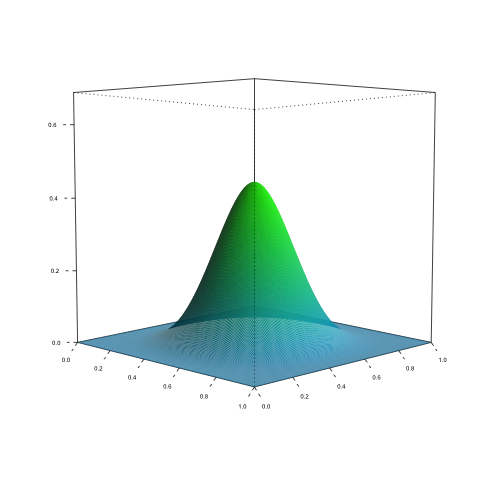
\includegraphics[width=4in, height=4in]{bicubic_bspline.png}
  \caption{Tensor product of two cubic B-splines}\label{fig:bicubic_bspline}
\end{figure}

\begin{figure}[H]
  \centering
  \graphicspath{{img/}}
  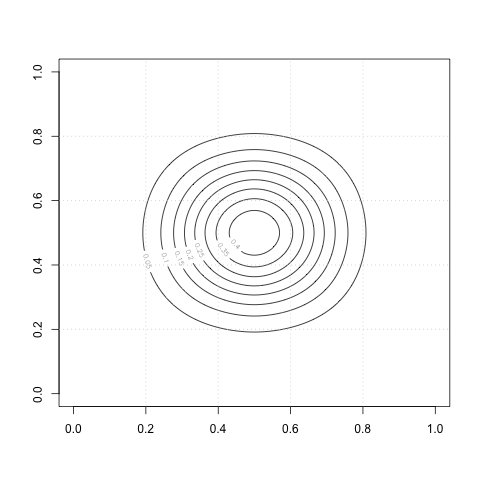
\includegraphics[width=4in, height=4in]{bicubic_bspline_contour.png}
  \caption{Tensor product of two cubic B-splines}\label{fig:bicubic_bspline_contour}
\end{figure} 

Temporarily focusing on a single axis, we first present some specific details of B-splines in the univariate case. 
\subsubsection{{\outlineskeleton Univariate B-splines}}

{\needsparaphrased B-splines are constructed from polynomial pieces, joined at certain values of the domain $t$, called knots. Once the knots are given, it is easy to compute the B-splines recursively, for any desired degree of the polynomial; see de Boor (1977, 1978), Cox (1981) or Dierckx (1993).  }

\begin{figure}[H]
  \centering
  \graphicspath{{img/}}
  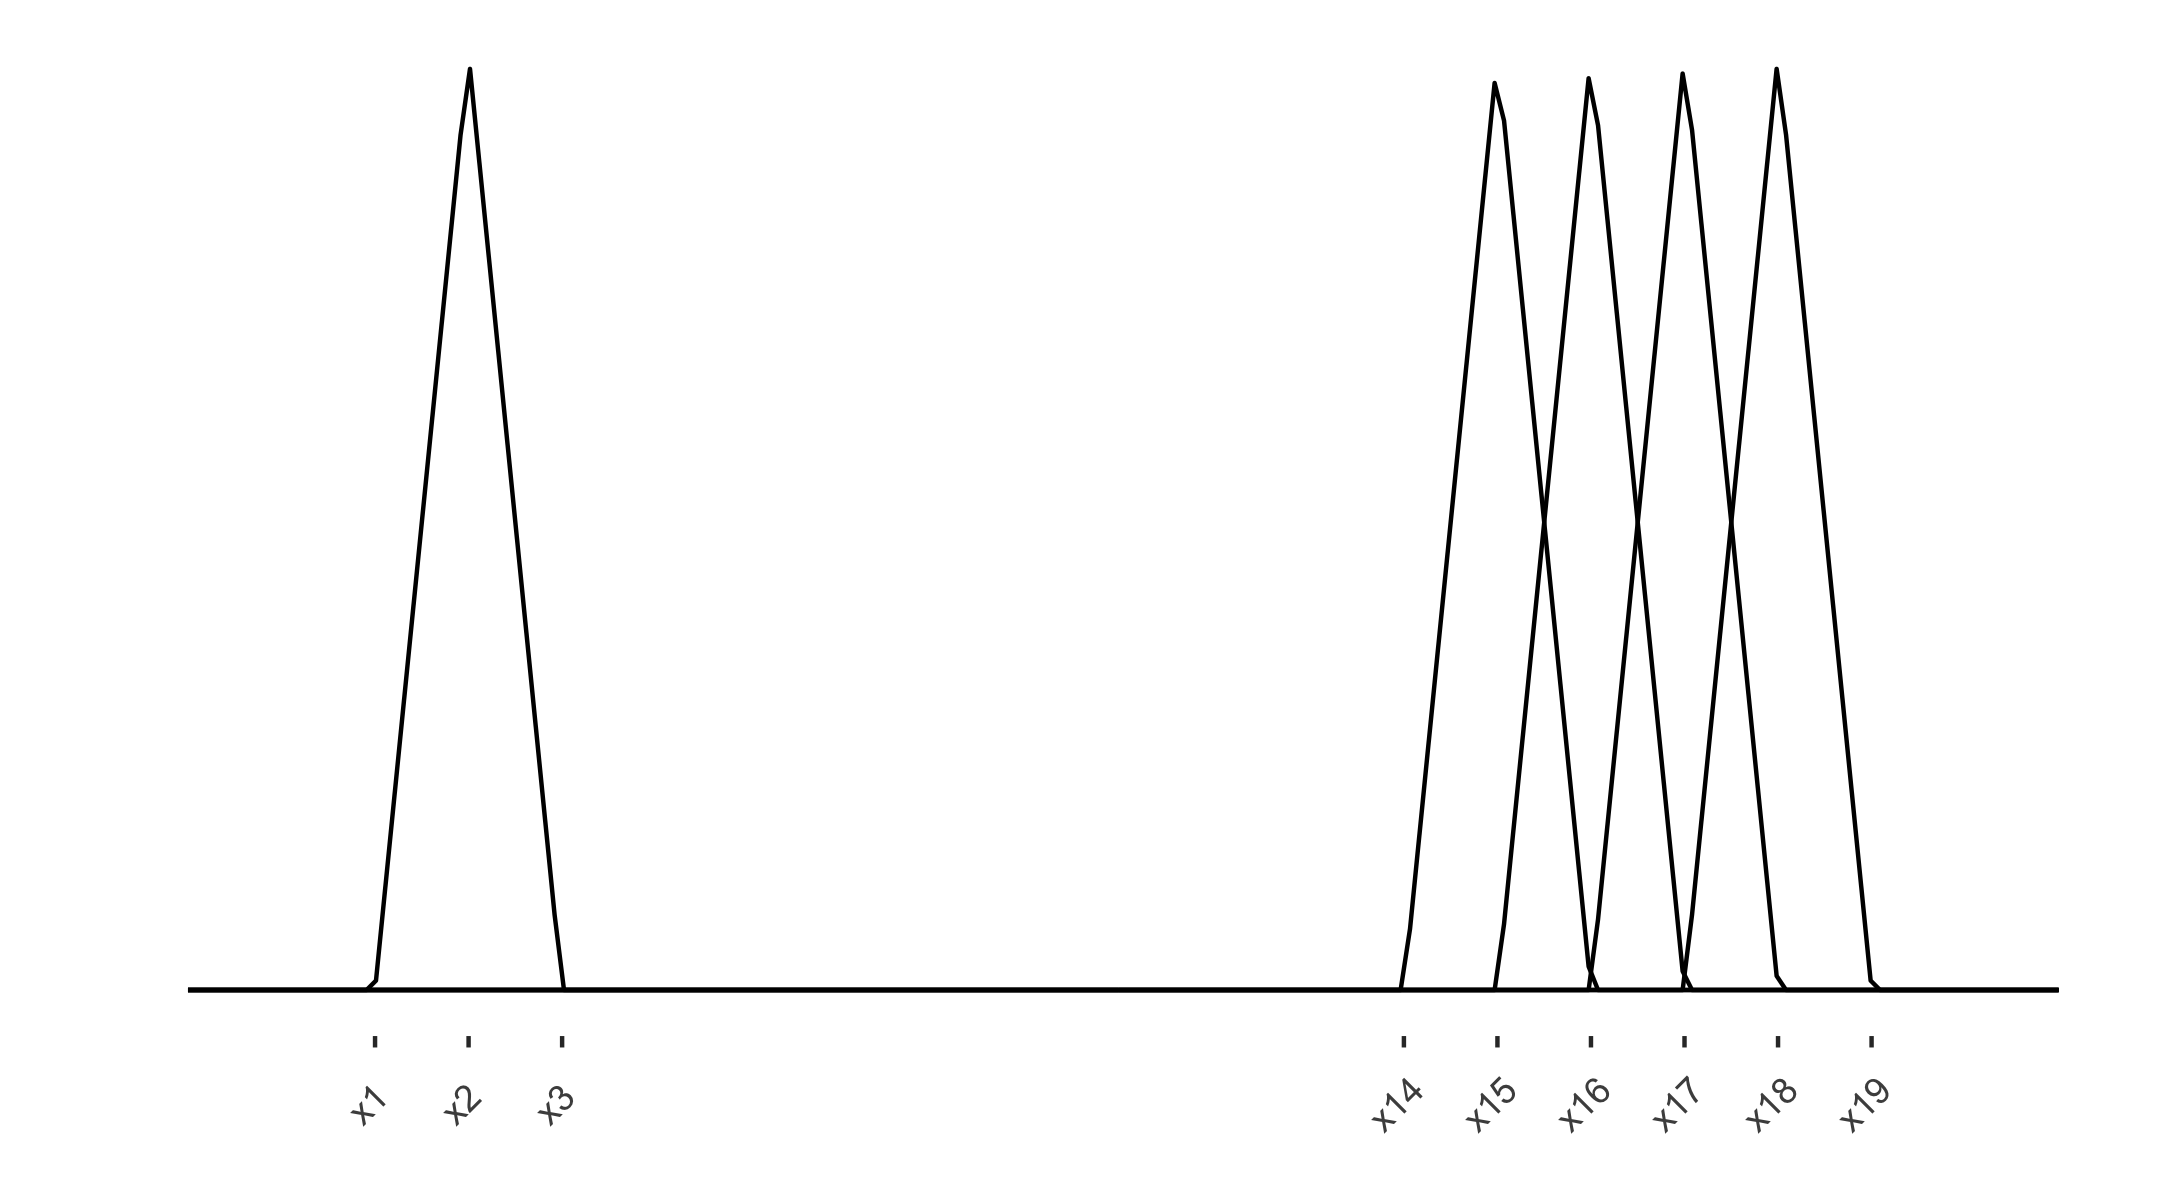
\includegraphics[width=3.7in, height=2.2in]{uni_linear_bsplines.png}
  \caption{B-splines of degree $q=1$}\label{fig:uni_linear_bsplines}
  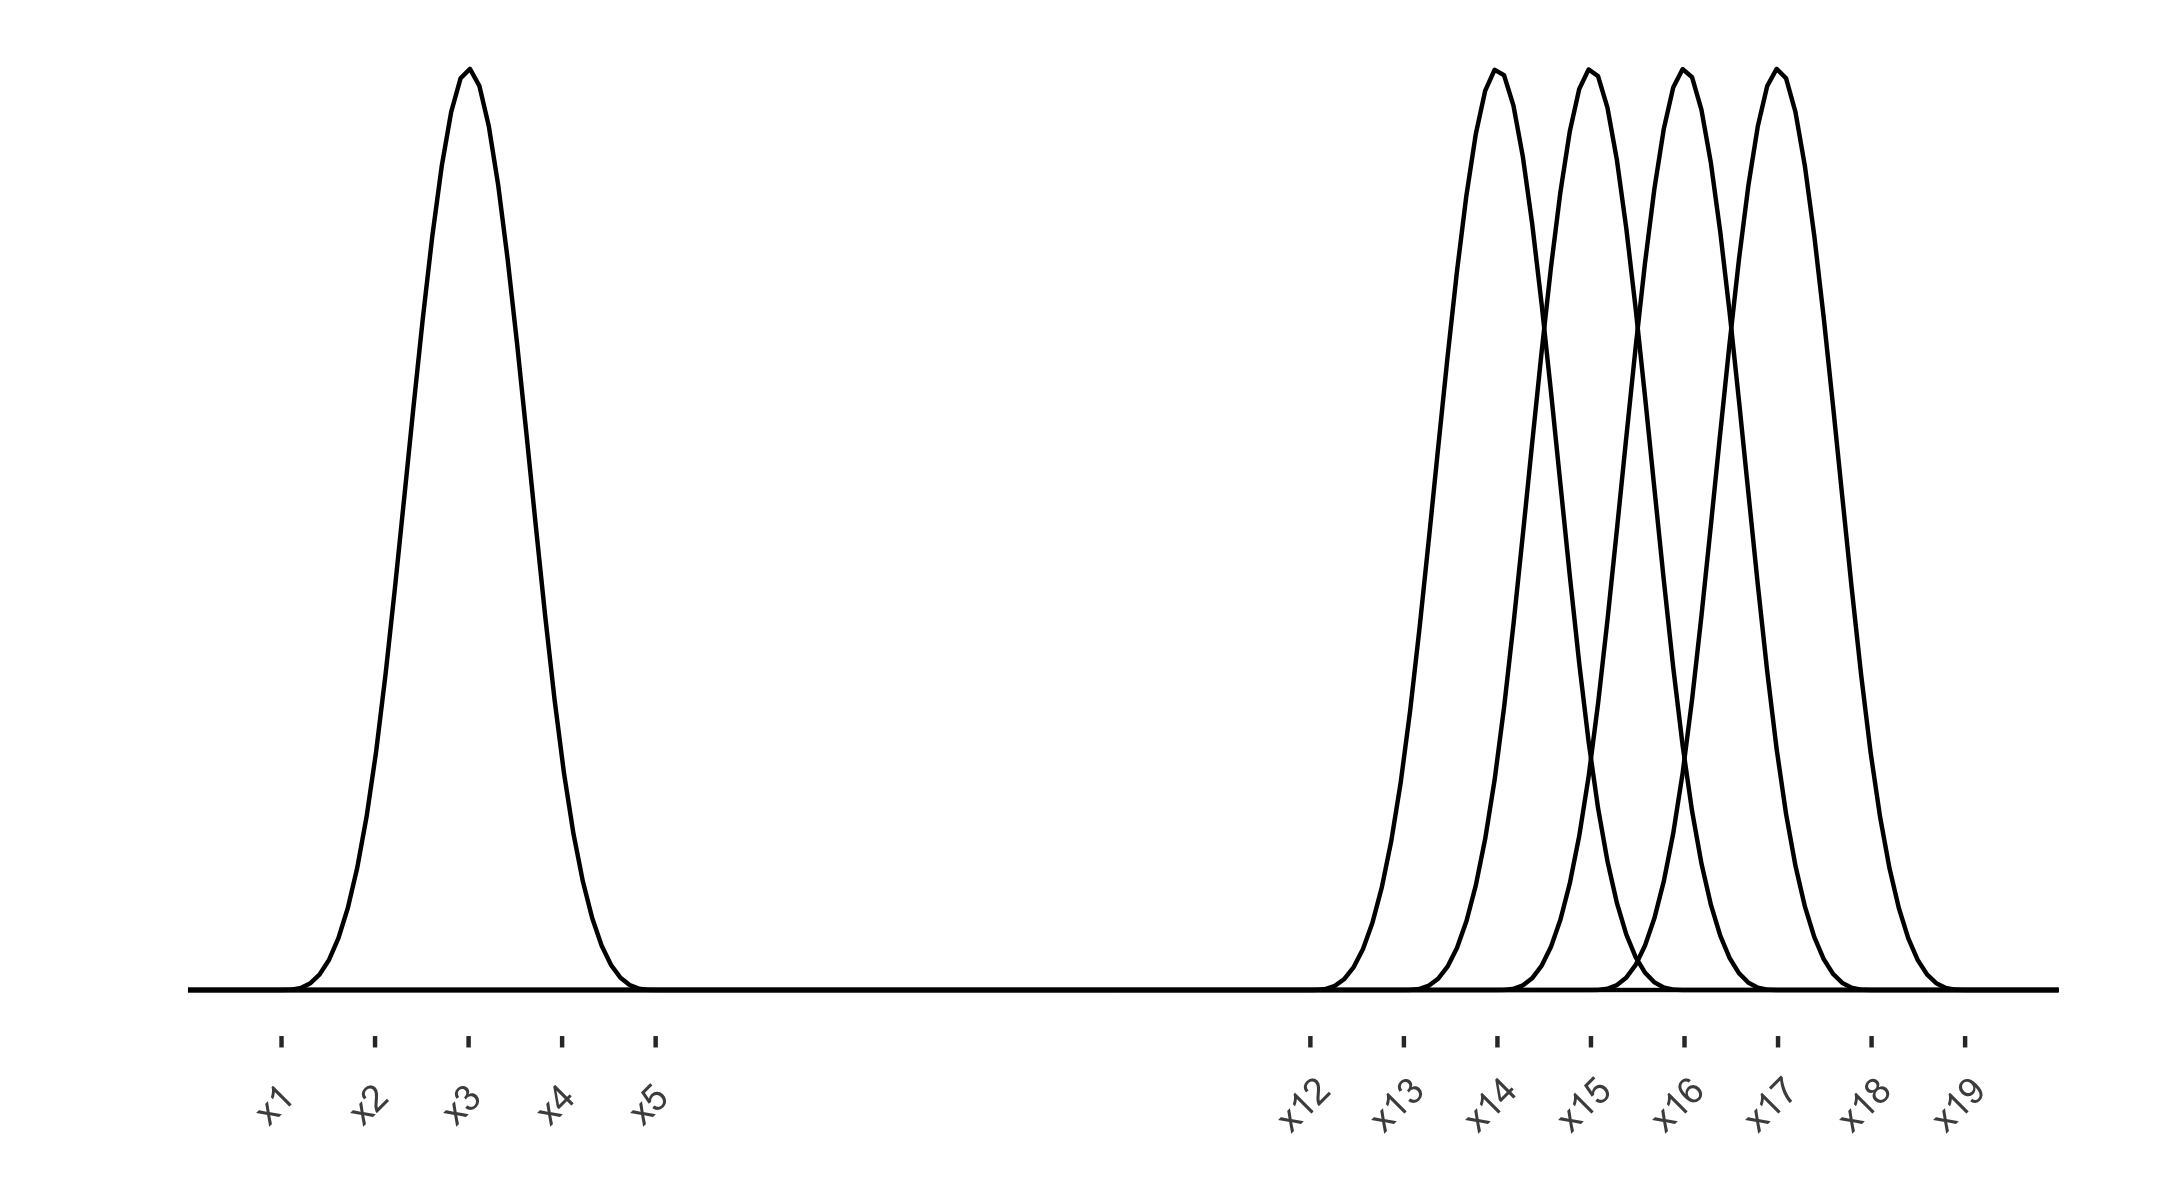
\includegraphics[width=3.7in, height=2.2in]{uni_cubic_bsplines.png}
  \caption{B-splines of degree $q=3$}\label{fig:uni_cubic_bsplines}
\end{figure} 

A B-spline consists of polynomial pieces connected in a particular way; a very simple example is shown in of Figure~\ref{fig:uni_linear_bsplines}: five linear B-splines. One the left is an isolated B-spline of degree 1; it consists of two linear pieces: one piece from $t_1$ to $t_2$, the other from $t_2$ to $t_3$. The knots are $t_1$, $t_2$, and $t_3$. To the left of $t_1$ and to the right of $t_3$, this B-spline takes value zero. To the right on the same axis, four more B-splines of degree 1 are shown: each one based on three knots. More B-splines are added to the collection with the introduction of additional knots.

Figure~\ref{fig:uni_cubic_bsplines} displays five B-splines of degree 3. It consists of four cubic pieces, joined at three inner knots. At the joining points of these cubic polynomials, not only the ordinates of the polynomial pieces match, but their first derivatives are also equal. (However, their second derivatives are not necessarily equal). The B-spline is based on five adjacent knots: $t_1,\dots,t_5$. To the right, four additional cubic B-splines are shown.

First-degree B-splines overlap with two neighbors, second-degree B-splines with four neighbors, and so on, with the leftmost and rightmost splines have being exceptions to this rule. At a given $t$, two first-degree (or four cubic) B-splines are nonzero. These examples illustrate the general properties of a B-spline of degree $q$:

\begin{itemize}
\item it consists of $q + 1$ polynomial pieces, each of degree q\\
\item the polynomial pieces join at $q$ inner knots\\
\item at the joining points, derivatives up to order $q - 1$ are continuous\\
\item the B-spline is positive on a domain spanned by $q +2$ knots; everywhere else it is zero\\
\item except at the boundaries, it overlaps with $2q$ polynomial pieces of its neighbors\\
\item at a given $t$, $q +1$ B-splines are nonzero.
\end{itemize}

Let $B_j^q\left(x\right)$ denote the $j^{th}$ B-spline of degree $q$. Expressions for the polynomial pieces may be derived by means of the following recursive relation:

\begin{align}
B_j^1\left(x\right) &= \left\{ \begin{array}{ll}
         1 & \mbox{if $x \in \left[x_i,x_{i+1}\right)$};\\
         0 & \mbox{otherwise}.\end{array} \right.\\
B_j^k\left(x\right) &= \frac{x-x_i}{x_{i+k-1}-x_i}B_j^{k-1}\left(x\right) + \frac{x_{i+k}-x}{x_{i+k}-x_{i+1}}B_{j+1}^{k-1}\left(x\right)         
\end{align}

We choose to divide the domain $t_{min}$ to $t_{max}$ into $n^\prime$ equal intervals, using $n^\prime +1$ interior knots. Taking each boundary into consideration, a complete basis needs $n^\prime + 2q + 1$ total knots, where $q$ is the degree of the B-spline. This is easily verified by constructing graphs like those in Figure~\ref{fig:uni_linear_cubic_bsplines}. B-splines are very attractive as basis functions for (``nonparametric'') univariate regression. A linear combination of, say, third-degree B-splines gives a smooth curve. Once one can compute the B-splines themselves, their application is no more difficult than polynomial regression.

Denote the knots as: $\phi_1,\dots ,\phi_{n^\prime+2q+1}$, and the collection of knots simply by $\phi$. The total number of B-splines on the axis is $n = n^\prime + q$. For indexing purposes it is convenient to associate each B-spline, $B_j\left(t\right)$ with exactly one of the $j = 1, \dots , n$ knots. We denote a full basis using matrix $B$, which has dimension $m \times n$. These basic properties comprise the essential background necessary for our pursuits, but for comprehensive treatment, we refer the reader to de Boor (1978) and Dierckx (1993).

{\needsparaphrased De Boor (1978)} presented an algorithm to compute B-splines of any degree from B-splines of lower degree. Because a zero-degree B-spline is just a constant on one interval between two knots, it is simple to compute B-splines of any degree. For the sake of simplicity in presentation, we only discuss the construction and properties given equidistant knots, but de Boor's algorithm also works for any placement of knots.

The indexing of B-splines needs some care, especially when we are going to use derivatives. The indexing connects a B-spline to a knot; that is, it gives the index of the knot that characterizes the position of the B-spline. Our choice is to take the leftmost knot, the knot at which the B-spline becomes nonzero. Let $B_j\left(t; q\right)$ denote the value at $t$ of the $j^{th}$ B-spline of degree $q$ for a given equidistant grid of knots. A fitted curve $\hat{y}$ to data $\left(t_i,y_i\right)$ is given by the linear combination $\hat{y}\left(t\right) = \sum_{j=1}^n \beta_{j} B_j\left(t; q\right)$. When the degree of the B-splines is clear from the context, or immaterial, we use $B_j\left(t\right)$ instead of $B_j\left(t; q\right)$.

De Boor (1978) gives a simple formula for derivatives of B-splines:
\begin{eqnarray}
h\sum_{j} \beta_j B_j^\prime \left(t,q\right) &=& \sum_{j} \beta_j B_j\left(t,q-1\right)-\sum_{j} \beta_{j+1} B_{j+1} \left(t,q-1\right) \nonumber \\ 
&=& -\sum_{j} \Delta\beta_{j+1} B_{j} \left(t,q-1\right) \label{bspline_deriv}
\end{eqnarray}
\noindent
where $h$ is the distance between knots and $\Delta \beta_j = \beta_j-\beta_{j-1}$. By induction, we have that the second derivative may be characterized as follows:
\begin{equation}
h^2\sum_{j} \beta_j B_j^{\prime \prime} \left(t,q\right) = \sum_{j} \Delta^2 \beta_{j} B_{j} \left(t,q-2\right) \label{bspline_2nd_deriv}
\end{equation}
\noindent
where $h$ is the distance between knots and $\Delta^2 \beta_j = \Delta\Delta \beta_j = \beta_j - 2\beta_{j-1}+\beta_{j-2} $. This fact is of particular utility when comparing continuous and discrete roughness penalties, which will follow in later discussion.



\subsubsection{{\outlineskeleton P-Splines Regularization}}

The smoothness of the curve fit to the data can be tuned with the number of B-splines in the basis; fewer knots (and hence basis functions) lead to smoother fits. This choice has been a subject of much research, as too many knots lead to overfitting while too few knots lead to underfitting. { \needsparaphrased Some authors have proposed automatic schemes for optimizing the number and the positions of the knots (Friedman and Silverman, 1989; Kooperberg and Stone, 1991,1992). This is a difficult numerical problem and, to our knowledge, no attractive all-purpose scheme exists.}

However, limiting the number of B-splines is not the only approach to achieving smoothness. Choosing an appropriate penalty on the coefficients of the basis functions can also achieve as much smoothness in the fitted function as desired. \cite{o1986statistical} was the first to propose using a rich B-spline basis and apply a discrete penalty to the spline coefficients. Using many B-splines allows one to sidestep the difficulty of choosing the optimal set of knots, while the penalty prevents overfitting and takes a potentially ill-conditioned fitting procedure to a well-conditioned one. He proposed a penalty on the second derivative to restrict the flexibility of the fitted curve, similar to the penalty pioneered for smoothing splines by Reinsch (1967). This penalty has become the standard in much of the spline literature; see Eubank (1988), Wahba (1990) and Green and Silverman (1994). This measure of roughness of a curve is given by 
 
 \[
 J = \int_l^u \left[ f^{\prime \prime}\left(x\right)\right]^2\;dx
 \]
 \noindent
 where $l$ and $u$ are the bounds on the domain of $x$. Using the properties of B-splines, if $f\left(x\right) = \sum_{j} \beta_j B_j\left(x\right)$, one can derive a banded matrix $P$ such that 
 \[
 J = \beta^\prime P \beta
 \] 
 \noindent
 where $\beta = \left(\beta_1,\dots, \beta_n\right)$, and the $i$-$j^{th}$ element of $P$ is given by
 \[
 p_{ij} = \int_l^u B_i^{\prime \prime} \left( x \right)B_j^{\prime \prime} \left( x \right)\;dx.
 \]
 \noindent
 He then proposed minimizing
 \begin{eqnarray*}
 Q\left(\beta, \lambda \right) &=& \sum_{i=1}^m \left(y_i - \sum_{j} \beta_j B_j\left(x_i \right)\right)^2 + \lambda \int_l^u \left[ f^{\prime \prime}\left(x\right)\right]^2\;dx\\
 &=& \vert \vert y - B\beta \vert  \vert^2 + \lambda\beta^\prime P \beta
 \end{eqnarray*}

The computation of $P$ is nontrivial and becomes very tedious when the third and fourth derivative are used as the roughness measure. \cite{wand2008semiparametric} extend O'Sullivan's work to higher order derivatives for general degree B-splines and derive an exact matrix algebraic expression for the penalty matrices. In the cubic case, the expression is a result of the application of Simpson's Rule applied to the inter-knot differences since each $B_i^{\prime \prime} B_j^{\prime \prime}$ is a piecewise quadratic function. The penalty may be written
 \[
 P = \left(B^{\prime \prime}\right)^\prime \textup{diag}\left(\omega \right) B^{\prime \prime}, 
 \]
 \noindent
 where $B^{\prime \prime}$ is the $3\left( n + 7 \right) \times \left( n + 4 \right)$ matrix with $i$-$j^{th}$ entry given by $B_j^{\prime \prime} \left(x_i^*\right)$, $x^*_i$ is the $i^{th}$ element of 
 
\[
\left( \phi_1,\frac{\phi_1+\phi_2}{2},\phi_2,\phi_2,frac{\phi_2+\phi_3}{2},\phi_3,\dots,\phi_{n+7},frac{\phi_{n+7}+\phi_{n+8}}{2},\phi_{n+8} \right),
\]
 \noindent
 and $\omega$ is the $3\left(n+7\right) \times 1$ vector given by
 
\begin{align*}
\omega &= \left( \frac{1}{6}\left(\Delta \phi \right)_1,\frac{4}{6}\left(\Delta \phi \right)_1, \frac{1}{6}\left(\Delta \phi \right)_1,\frac{1}{6}\left(\Delta \phi \right)_2, \frac{4}{6}\left(\Delta \phi \right)_2,  \right. \\
&\qquad   \left. {} \frac{1}{6}\left(\Delta \phi \right)_2 , \dots , \frac{1}{6}\left(\Delta \phi \right)_{n+7}, \frac{4}{6}\left(\Delta \phi \right)_{n+7}, \frac{1}{6}\left(\Delta \phi \right)_{n+7}  \right) \\
\end{align*}
\noindent
 where $\left(\Delta \phi \right)_j = \phi_{j+1}-\phi_j$. They generalize this to the case of any order penalty and present a table of formulas for constructing any arbitrary penalty matrix, $P$.
 
 {\needsparaphrased  \cite{eilers1996flexible} simplify and generalize the approach of O'Sullivan, in such a way that it can be applied in any context where regression on B-splines is useful. }They present P-splines as an approach to nonparametric smoothing; they circumvent any complexity associated with constructing such penalty matrices by discarding derivatives and integrals altogether. Instead, they use a discrete penalty matrix which is simple to compute, as it is based on difference formulas. Let 
 
 \begin{eqnarray*}
 \Delta \beta_j &=& \beta_j - \beta_{j-1},\\
 \Delta^2 \beta_j &=& \Delta\left(\Delta \beta_j\right) = \beta_j - 2\beta_{j-1} + \beta_{j-2},\\ 
 \end{eqnarray*}
\noindent 
and in general,
\begin{equation*}
\Delta^d \beta_j = \Delta\left(\Delta^{d-1} \beta_j \right)
\end{equation*}
 Let $D_d$ denote the matrix difference operator; that is, $D_d\beta = \Delta^d \beta$. Replacing O'Sullivan's penalty with 
 \[
 \lambda\vert \vert D_d\beta\vert \vert^2 = \lambda \beta^\prime D^\prime_d D_d \beta = \lambda \beta^\prime P\beta,
 \] 
 \noindent
yields a similar construction as O?Sullivan?s, but with minimal effort required to implement the penalty. It can be shown with relative ease that nothing is lost by using the simplified penalty, and that for second order differences, Marx and Eilers' P-spline approach is very similar to that of O'Sullivan. Details will be presented in the section to immediately follow.
 
 In some applications, however, it can be useful to use differences of a smaller or higher order in the penalty. The P-spline smoothing approach allows for ease of incorporation of a penalty of any order in the regression equations. 

\subsubsection{{\outlineskeleton P-Spline Difference Penalties for Univariate B-Splines}} \label{uni_pspline_penalties}

Consider the regression of $m$ data points $\left(t_i,y_i\right)$ on a set of $n$ B-splines $B_j$. The least squares objective function to minimize is

\begin{equation} \label{eq:univariate_bspline_SSE}
\sum_{i=1}^m \left\{ y_i - \sum_{j=1}^n \beta_j B_j\left(t_i\right) \right\}^2
\end{equation}
\noindent

{ \needsparaphrased Let the number of knots be relatively large, such that the fitted curve will show more variation than is justified by the data. To make the result less flexible, O'Sullivan (1986, 1988) introduced a penalty on the second derivative of the fitted curve and so formed the objective function}

\begin{equation} \label{eq:univariate_bspline_ridge_penalty}
\sum_{i=1}^m \left \{ y_i - \sum_{j=1}^n \beta_j B_j\left(t_i\right) \right \}^2 + \lambda \int_{t_{min}}^{t_{max}} \left\{  \sum_{j=1}^n \beta_j B^{\prime \prime}_j\left(t\right) \right\}^2 \; dt
\end{equation}



{ \needsparaphrased The integral of the square of the second derivative of a fitted function has become common as a smoothness penalty, since the seminal work on smoothing splines by Reinsch (1967). There is nothing special about the second derivative; in fact, lower or higher orders might be used as well. In the context of smoothing splines, the first derivative leads to simple equations, and a piecewise linear fit, while higher derivatives lead to rather complex mathematics, systems of equations with a high bandwidth, and a very smooth fit. \cite{eilers1996flexible} propose to base the penalty on (higher-order) finite differences of the coefficients of adjacent B-splines:}

\begin{equation} \label{eq:univariate_pspline_diff_penalty}
\sum_{i=1}^m \left \{ y_i - \sum_{j=1}^n \beta_j B_j\left(t_i\right) \right \}^2 + \lambda \sum_{j=k+1}^n \left( \Delta^k \beta_j  \right)^2
\end{equation}

This approach reduces the dimensionality of the problem to the number of B-splines, $n$ instead of the number of observations, $m$ , as with smoothing splines. The tuning parameter $\lambda$ permits continuous control over smoothness of the fit. We will demonstrate that the difference penalty is a good discrete approximation to the integrated square of the $k^{th}$ derivative, and with this penalty, moments of the data are conserved and polynomial regression models occur as limits for large values of $\lambda$. We will explore the connection between a penalty on second-order differences of the B-spline coefficients and O'Sullivan's choice of a penalty on the second derivative of the fitted function. However, the difference penalty can be handled mechanically for any order of the differences.

{ \needsparaphrased Difference penalties have a long history that goes back at least to Whittaker (1923); recent applications have been described by Green and Yandell (1985) and \cite{eilers1991penalized}, \cite{eilers1991nonparametric}, \cite{eilers1995indirect}. The difference penalty is easily introduced into the regression equations. That makes it possible to experiment with different orders of the differences. In some cases it is useful to work with even the fourth or higher order. This stems from the fact that for high values of $\lambda$ the fitted curve approaches a parametric (polynomial) model, as will be shown below.
\cite{o1986statistical} used third-degree B-splines and the following penalty:}

\begin{equation} \label{eq:osullivan_univariate_bspline_penalty}
h^2 P = \lambda \int_{t_{min}}^{t_max} \left\{ \sum_{j}  \beta_j B_j^{\prime \prime} \left(t, q=3\right) \right\}^2\; dt
\end{equation}
\noindent
From the derivative properties of B-splines, it follows that

\begin{equation} \label{osullivan_univariate_bspline_penalty_via_deriv}
h^2 P = \lambda \int_{t_{min}}^{t_max}  \sum_{j} \sum_{k} \Delta^2 \beta_j \Delta^2 \beta_k B_j\left(t,q=1\right)B_k\left(t,q=1\right) dt 
\end{equation}
\noindent
Most of the cross products of $B_j(t; 1)$ and $B_k(t;1)$ vanish as B-splines of degree 1 only overlap when $j$ is $k-1$, $k$, or $k+1$. Thus, we have that

\begin{align}
h^2 P = {} & \lambda \int_{t_{min}}^{t_{max}} \bigg[ \left\{ \sum_{j}  \Delta^2 \beta_j  B_j\left(t,1\right)  \right\}^2  + 2 \sum_{j}\Delta^2 \beta_j\Delta^2 \beta_{j-1}B_j\left(t,1\right)B_{j-1}\left(t,1\right) \bigg] dt \nonumber \\ 
= {} & \lambda \bigg[ \sum_j \left( \Delta^2\beta_j \right)^2 \int_{t_{min}}^{t_{max}} B_j^2\left(t,1\right)\;dt + 2 \sum_j \Delta^2 \beta_j\Delta^2 \beta_{j-1} \bigg]
\end{align}
\noindent
or
\begin{align}
h^2 P = \lambda \sum_j \left( \Delta^2\beta_j \right)^2 \int_{t_{min}}^{t_{max}} B_j^2\left(t,1\right) dt + {} & 2\lambda \sum_j \Delta^2 \beta_j \Delta^2 \beta_{j-1}  \nonumber \\ 
{} &+\int_{t_{min}}^{t_{max}} B_j\left(t,1\right)B_{j-1}\left(t,1\right) dt
\end{align}
\noindent
which can be written as
\begin{equation} \label{eq:osullivan_penalty_decomp}
h^2 P = \lambda\left\{c_1 \sum_j\left( \Delta^2 \beta_j\right)^2 + c_2 \sum_j\Delta^2 \beta_j\Delta^2 \beta_{j-1} \right\}
\end{equation}
\noindent
where, for given equidistant knots, $c_1$ and $c_2$ are constants given by
\begin{equation}
\begin{split}
c_1 & =   \int_{t_{min}}^{t_{max}} B_j^2\left(t,1\right) dt\\
c_2 & = \int_{t_{min}}^{t_{max}} B_j\left(t,1\right)B_{j-1}\left(t,1\right) dt
\end{split}
\end{equation}

Thus, we see that O'Sullivan's ridge-like B-spline penalty \ref{eq:osullivan_univariate_bspline_penalty} can be written as a linear combination of Marx and Eilers' difference penalty \ref{eq:univariate_pspline_diff_penalty} and the sum of the cross products of neighboring second differences. The second term in \ref{eq:osullivan_penalty_decomp} leads to a complex objective function when minimizing the penalized likelihood, where seven adjacent spline coefficients occur, as opposed to five if only the first term in \ref{eq:osullivan_penalty_decomp} is used in the penalty. The added complexity is a consequence of overlapping B-splines, and these complexities grow quickly with higher order differences and B-splines of higher degree, which makes it difficult to construct a procedure for incorporating the penalty in the likelihood equations. Using a difference penalty allows us to sidestep this complexity.

Using the sum of squared errors as the goodness of fit measure, we define $\hat{\beta} = \left(\beta_1, \beta_2, \dots, \beta_n \right)$ to be the minimizer of
\begin{equation*}  
S_\lambda\left(y, \beta \right) = \sum_{i=1}^m \left\{ y_i - \sum_{j=1}^K \beta_j B_j\left(t_i\right) \right\}^2 + \lambda \sum_{j=k+1}^n \left( \Delta^k\beta_j \right)^2
\end{equation*}
\noindent
In vector notation, this may be written
\begin{equation}\label{eq:uni_pspline_penalized_likelihood}
S_\lambda \left(y, \beta \right) = \left( y- B\beta  \right)^T \left( y-B \beta\right) + \lambda \left(D_k \beta\right)^T\left(D_k \beta\right)
\end{equation}
\noindent
where $D_k$ is the matrix difference operator $\Delta_k$,and the elements of $B$ are $b_{ij} = B_j\left(t_i\right)$ as defined . Taking derivatives on both sides of \ref{eq:uni_pspline_penalized_likelihood} with respect to $\beta$ gives
\begin{align}
\frac{\partial}{\partial \beta}\left(L\left(Y, \beta \right) + \lambda J\left(\beta\right) \right) ={} & \frac{\partial}{\partial \beta}\left(\beta^TB^TB \beta -2Y^T B^T\beta+\lambda \beta^T D_k^T D_k \beta  \right) \nonumber \\
= {} & 2B^TB \beta - 2B^T Y + 2\lambda D_k^TD_k\beta \nonumber\\
= {} & \left(B^T B +  \lambda D_k^TD_k\right)\beta - B^T Y \label{eq:uni_penalized_lik_deriv}
\end{align} 
\noindent
Setting \ref{eq:uni_penalized_lik_deriv} equal to zero yields the following normal equations:
\begin{equation}\label{eq:uni_pspline_normal_eq}
B^T Y = \left(B^T B +  \lambda D_k^TD_k\right)\beta
\end{equation}
When $\lambda = 0$, we have the standard normal equations of linear regression with a B-spline basis, and with $k = 0$ \ref{eq:uni_pspline_normal_eq} corresponds to the normal equations under the ridge regression penalty. When $\lambda > 0$, the penalty only influences the main diagonal and $k$ subdiagonals of the system of equations. This system has a banded structure because of the limited overlap of the B-splines, though exploiting this special structure is of little utility since the number of equations is equal to the number of splines, which is generally moderate. 


\subsubsection{{\outlineskeleton Properties of P-Splines}}

{\needsparaphrased 
\large [ Discussion of B-splines as defined by their coefficients - see BS section 4.2 IV] 
}

{\needsparaphrased A fruitful way of looking at P-splines is to give the coefficients a central position as a skeleton, with the B-splines merely putting ``the flesh on the bones.'' This is illustrated
in Figure~\ref{fig:psplines_second_ord_pen_SML_lambda}. A smoother sequence of coefficients leads to a smoother curve. The number of splines and coefficients is immaterial, as long as the latter are smooth. The role of the penalty is to make such happen. }

\begin{figure}[H]
\begin{subfigure}{.5\textwidth}
  \centering
   \graphicspath{{img/}}
  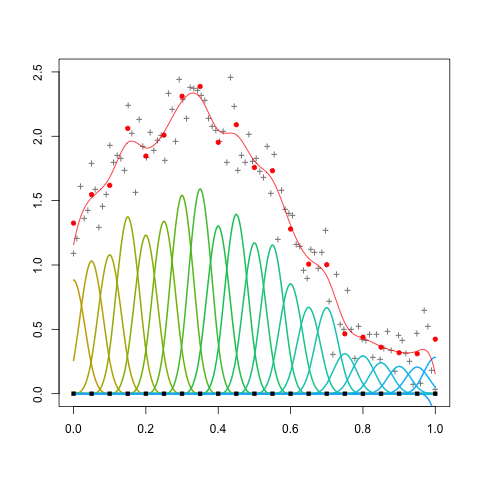
\includegraphics[scale=0.5]{pspline_pord2_xsmall_lambda.png}
  \label{fig:pspline_small_lambda}
\end{subfigure}
\begin{subfigure}{.5\textwidth}
  \centering
   \graphicspath{{img/}}
  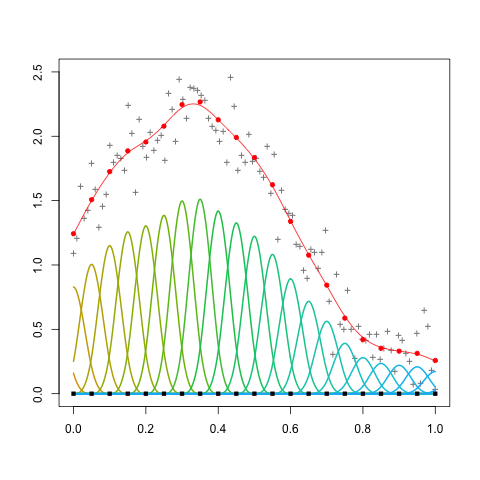
\includegraphics[scale=0.5]{pspline_pord2_small_lambda.png}
  \label{fig:pspline_small_lambda}
\end{subfigure}
\begin{subfigure}{.5\textwidth}
  \centering
   \graphicspath{{img/}}
  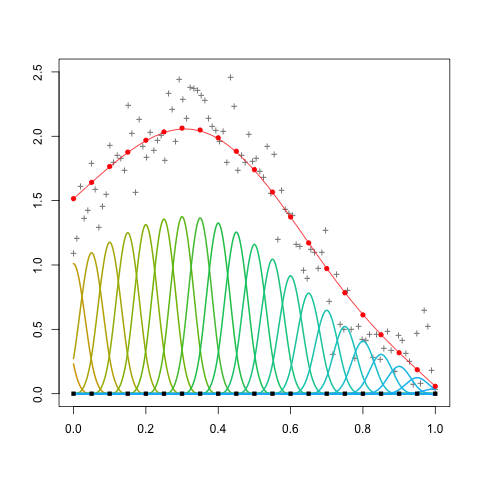
\includegraphics[scale=0.5]{pspline_pord2_medium_lambda.png}
  \label{fig:pspline_small_lambda}
\end{subfigure}
\begin{subfigure}{.5\textwidth}
  \centering
   \graphicspath{{img/}}
  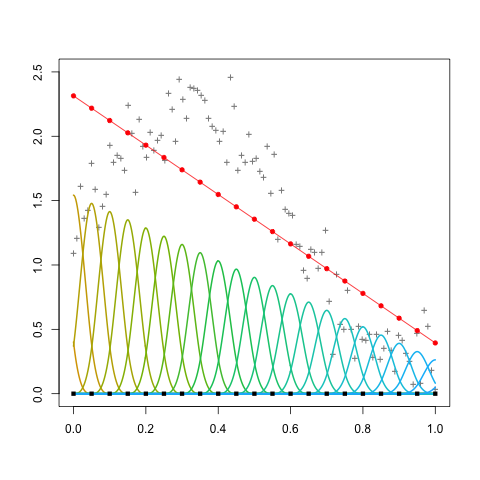
\includegraphics[scale=0.5]{pspline_pord2_large_lambda.png}
  \label{fig:pspline_small_lambda}
\end{subfigure}
\caption{\textit{Illustration of the impact of the second order difference penalty. The number of B-splines used is the same in each plot, with the value of the penalty parameter increasing from left to right and top to bottom across each plot. The fitted curve in the upper left plot is the most ``wiggly'' of any of the fits, as the penalty plays the weakest roll in the fitted coefficients there. The red circles are the values of each of the B-spline coefficients; as the penalty increases, they form as smoother sequence as we move across the four plots, which results in a smoother fitted function. As the penalty parameter approaches infinity, the fit approaches a linear function as shown in the bottom right plot.}}
\label{fig:psplines_second_ord_pen_SML_lambda}
\end{figure}

{\needsparaphrased The number of B-splines can be (much) larger than the number of observations. The penalty makes the fitting procedure well-conditioned. This should be taken literally: even a thousand splines will fit ten observations without problems. Such is the power of the penalty. Figure~\ref{fig:overcomplete_basis_pspline} illustrates this for simulated data. There are 10 data points and 40 (+3) cubic B-splines. Unfortunately, this property of P-splines (and other types of penalized splines) is not generally appreciated. But one simply cannot have too many B-splines. A wise choice is to use 100 of them, unless computational constraints (in large models) come into sight. We will return to this example in Section 4, after introducing the effective model dimension, and further address this issue of many splines in Appendix B.}

\begin{figure}[H]   \label{fig:overcomplete_basis_pspline}
  \centering
   \graphicspath{{img/}}
  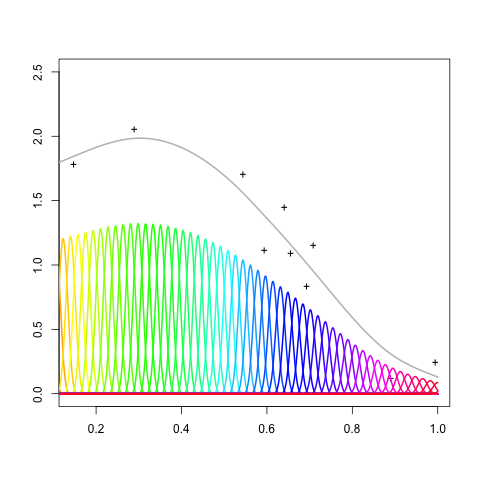
\includegraphics[scale=0.75]{pspline_10obs_60_basis_functions.png}
  \caption{P-spline smoothing of 10 observations using 60 B-spline basis functions.}
\end{figure}


{\needsparaphrased P-splines have a number of useful properties, partially inherited from B-splines. We give a short overview, with somewhat informal proofs. In the first place: P-splines show no boundary effects, as many types of kernel smoothers do. By this, we mean the spreading of a fitted curve or density outside of the (physical) domain of the data, generally accompanied by bending toward zero. In Section 8 this aspect is considered in some detail, in the context of density smoothing. }

P-splines can fit polynomial data exactly. Let data $\left(t_i,y_i\right)$ be given. {\needsproof If the $y_i$ are a polynomial in $t$ of degree $k$, then B-splines of degree $k$ or higher will exactly fit the data (de Boor, 1977).}The same is true for P-splines, if the order of the penalty is $k +1$ or higher, whatever the value of $\lambda$. To see that this is true, take the case of a first-order penalty and the fit to data $y$ that are constant (a polynomial of degree 0). Note that 
\[
\sum_{j=1}^n \hat{\beta}_j B_j\left( x_i \right) = c, 
\]
\noindent
and consequently, we have 
\[
\sum_{j=1}^n \hat{\beta}_j B^\prime_j\left( x \right) = 0, 
\]
\noindent
for all $x$. From the relationship between differences and derivatives in \ref{eq:bspline_deriv}, 

\[
0 = h \sum_{j=1}^n \beta^\prime_j\left(x, q\right) = \sum_{j=1}^n \Delta\beta_{j+1} B_j\left(x, q-1\right), 
\]
\noindent
so that we must have $\Delta \beta_j = 0$ for all $j$, and 
\[
\sum_{j=2}^n \Delta \beta = 0.
\]

Hence there is no impact of the penalty on the basis coefficients, making the fit identical to that when using unpenalized B-splines. Similarly, one can show using an inductive argument that this is also true when the relationship between $x$ and $y$ is linear and a second order difference penalty is used. Consequently, the penalty has no effect and the fit is the same as for unpenalized B-splines. This reasoning can easily be extended by induction to data with a linear relationship between $x$ and $y$, and a second order difference penalty. 



P-splines can conserve moments of the data. For a linear model with P-splines of degree k +1 and a penalty of order k +1,or higher, it holds that 

{\needsparaphrased  for all values of A, where 5i= C)=lbUfj are the fit- ted values. For GLM's with canonical links it holds that }

{\needsparaphrased This property is especially useful in the context of density smoothing: the mean and variance of the estimated density will be equal to mean and variance of the data, for any amount of smoothing. This is an advantage compared to kernel smoothers: these inflate the variance increasingly with stronger smoothing. The limit of a P-splines fit with strong smoothing is a polynomial. For large values of $\lambda$ and a penalty of order $k$, the fitted series will approach a polynomial of degree $k-1$, if the degree of the B-splines is equal to, or higher than, $k$. Once again, the relationships between derivatives of a B-spline fit and differences of coefficients, as in (1) and (2), are the key. Take the example of a second-order difference penalty: when $h$ is large, Cy=3(A2aj ) 2 has to be very near zero. Thus each of the second differences has to be near zero, and thus the second derivative of the fit has to be near zero everywhere. In view of these very useful results, it seems that B-splines and difference penalties are the ideal marriage.

It is important to focus on the linearized smoothing problem that is solved at each iteration, because we will make use of properties of the smoothing matrix. From (16) follows for the hat matrix $H$:}

{\needsparaphrased The trace of $H$ approaches $k$ as $\lambda$ increases. A proof goes as follows: let...}

\subsubsection{{\outlineskeleton Model Selection and Tuning}}

A major problem of any smoothing technique is the choice of the optimal amount of smoothing; now that it is established how we can easily influence the smoothness of a fitted curve with $\lambda$, there is need for some method of choosing an "optimal" value for it. Two potential model selection criteria are cross-validation and the Akaike information criterion (AIC). The latter is effectively a correction to the log likelihood to adjust for the effective dimension, or the effective number of parameters in the model. We choose to follow in the approach of\cite{eilers1996flexible}, \cite{marx2005multidimensional}, and \cite{buja1989linear} in using the trace of the smoother matrix as the effective dimension. This quantity is easily computed with the use of standard regression techniques, and is useful to compare the effective amount of smoothing for different numbers of knots, different degrees of the B-splines and different orders of penalties.

{\needsparaphrased  We propose to use the Akaike information criterion (AIC). The basic idea.of AIC is to correct the log- likelihood of a fitted model for the effective number of parameters. An extensive discussion and applications can be found in Sakamoto, Ishiguro and Kitagawa (1986). Instead of the log-likelihood, the deviance is easier to use. The definition of AIC is equivalent to}

{\needsparaphrased where dim(a, A) is the (effective) dimension of the vector of parameters, a , and dev(y; a , A) is the deviance.
Computation of the deviance is straightforward, but how shall we determine the effective dimension of our P-spline fit? We find a solution in Hastie and Tibshirani (1990). They discuss the effective dimensions of linear smoother and propose to use the trace of the smoother matrix as an approximation. In our case that means dim(a) = tr(H). Note that $tr\left(H\right) = n$ when $\lambda = 0$, as in (nonsingular) standard linear regression. 

As $tr\left(AB\right) = tr\left(BA\right)$ (for conformable matrices), it is computationally advantageous to use}

{\needsparaphrased The latter expression involves only n-by-n matrices, whereas $H$ is an $m \times m$ matrix. An estimate of the variance is needed, and one approach is to take the variance of the residuals from the $\hat{y}_i$ that are computed when $\lambda = 0$, say, $\hat{\sigma}_0^2$:}

\begin{equation} \label{eq:univariate_AIC}
\textup{AIC}\left(\lambda\right) = \sum_{i=1}^m \frac{\left( y_i - \hat{\mu}_i \right)^2}{\hat{\sigma}_0^2} + 2tr\left(H\right) - 2m\log\left(\hat{\sigma}_0\right) - m\log 2\pi
\end{equation}

{\needsparaphrased This choice for the variance is rather arbitrary, as it depends on the number of knots. Alternatives can be based on (generalized) cross-validation. For ordinary cross-validation we compute}
\begin{equation} \label{eq:univariate_CV}
\textup{CV}\left(\lambda\right) = \sum_{i=1}^m \left( \frac{ y_i - \hat{y}_i }{1-h_{ii}}\right)^2 
\end{equation}
{\needsparaphrased where the $h_{ii}$ are the diagonal elements of the hat matrix, $H$. For generalized cross-validation (Wahba, 1990), we compute }
\begin{equation} \label{eq:univariate_GCV}
\textup{GCV}\left(\lambda\right) = \sum_{i=1}^m \frac{\left(  y_i - \hat{y}_i \right)^2}{\left(m-\sum_{j=1}^m h_{jj}\right)^2} 
\end{equation}
{\needsparaphrased The difference between both quantities is generally small. The best $\lambda$ is the value that minimizes $\textup{CV}\left(\lambda\right)$ or $\textup{GCV}\left(\lambda\right) $. The variance of the residuals at the optimal $\lambda$ is a natural choice to use as an estimate of $\hat{\sigma}_0^2$ for the computation of $\textup{AIC}\left(\lambda\right)$. It is practical to work with modified versions of $\textup{CV}\left(\lambda\right)$ and $\textup{GCV}\left(\lambda\right)$, with values that can be interpreted as estimates of the cross-validation standard deviation:}

\begin{equation}
\begin{split}
\bar{\textup{CV}\left(\lambda\right)} &= \sqrt{m^{-1}\textup{CV}\left(\lambda\right)} \\
\bar{\textup{GCV}\left(\lambda\right)} &= \sqrt{m\textup{GCV}\left(\lambda\right)} \\
\end{split}
\end{equation}

{\needsparaphrased The two terms in $\textup{AIC}\left(\lambda\right)$ represent the deviance and the trace of the smoother matrix, respectively. The latter term, say $T\left(\lambda\right) = tr\left(H\left(\lambda\right)\right)$, is of interest on its own, because it can be interpreted as the effective dimension of the fitted curve.

$T\left(\lambda\right)$ is useful to compare fits for different numbers of knots and orders of penalties, whereas $\lambda$ can vary over a large range of values and has no clear intuitive appeal. We will show in an example below that a plot of $\textup{AIC}$ against $T$ is a useful diagnostic tool. In the case of P-splines, the maximum value that $T\left(\lambda\right)$ can attain is equal to the number of B-splines (when $\lambda = 0$). The actual maximum depends on the number and the distributions of the data points. The minimum value of $T\left(\lambda\right)$ occurs when $\lambda$ goes to infinity and is equal to the order of the difference penalty. This agrees with the fact that for high values of $\lambda$, the fit of P-splines approaches a polynomial of degree $k - 1$.}



\subsection{{\outlineskeleton Tensor Product B-splines}}

Tensor product B-splines exist in the $t \times \tilde{t}$ plane. For our presentation, $n$ ($\tilde{n}$) equally-spaced indexing knots are placed on the $t$ ($\tilde{t}$) axis to yield a regularly-spaced grid, carving out the plane into sub-rectangles. The $r^{th}-s^{th}$ single tensor product $B_r\left(t\right)$ ($B_s\left(\tilde{t}\right)$), as presented in Figure~\ref{fig:bicubic_bspline} and Figure~\ref{fig:bicubic_bspline_contour}, is positive in the rectangular region defined by the knots $R = \left[\phi_r, \phi_{r+q+2}\right] \times \left[\tilde{\phi}_s, \tilde{\phi}_{s+\tilde{q}+2}\right]$ or on a support of spanned by $\left(q + 2\right) \times \left(\tilde{q} + 2\right)$ knots. Similar to univariate B-splines, we index each tensor product by one of the $n\times\tilde{n}$ knot pairs, where

\begin{equation} \nonumber
\begin{split}
B_r\left(\tilde{t}\right)B_s\left(\tilde{t}\right) & > 0 \;\; \textup{for all }  t,\; \tilde{t}\;\ \in R\\
 & = 0 \;\; \textup{for all }  t,\; \tilde{t}\;\ \not\in R
\end{split}
\end{equation}
\noindent
for $r = 1,\dots, n$, $s = 1,\dots, \tilde{n}$. Figure~\ref{fig:sparse_bicubic_basis} displays nine tensor product B-splines, which represents only a portion of a full basis. A graphic of a complete basis would be of little illustrative use, as the``hills'' overlap quite a lot, making each individual basis function difficult to isolate from the rest. Associated with each ``hill'' in Figure~\ref{fig:sparse_bicubic_basis} , there is an unknown coefficient. 

The complete tensor product B-spline basis thus has an unknown coefficient matrix, denoted by $\Gamma_{n\times\tilde{n}} = \left[\gamma_{rs}\right]$. For given knot grid, a very flexible surface can be approximated, e.g. at the digitized coordinates. For $j=1,\dots,p$ and $k=1,\dots,\tilde{p}$,
\begin{equation} \label{eq:coefficient_surface_expansion}
\alpha\left(t_{j}, \tilde{t}_{k}\right) = \sum_{r=1}^n \sum_{s=1}^{\tilde{n}}  B_r\left(t_{j}\right) B_s\left(\tilde{t}_{k}\right) \gamma_{rs}
\end{equation}
\noindent
The surface is defined by relatively few parameters $\left(n \tilde{n} \right)$, where changing $\Gamma$ implies changes the surface.

\begin{figure}[H]
\begin{subfigure}
  \centering
 \graphicspath{{img/}}
  \includegraphics[width=4in, height=4in]{bicubic_bspline_mesh.png}
  \label{fig:bicubic_bspline}
\end{subfigure}

\begin{subfigure}
  \centering
  \graphicspath{{img/}}
  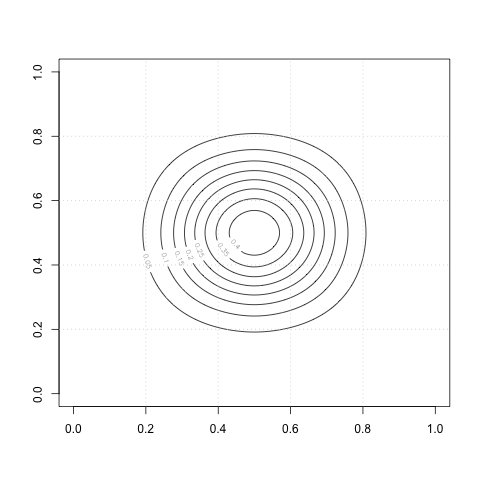
\includegraphics[width=4in, height=4in]{bicubic_bspline_contour.png}
  \caption{Tensor product of two cubic B-splines}\label{fig:bicubic_bspline_contour}
\end{subfigure}
\label{fig:bicubic_BS}
\end{figure}

%Figure~\ref{fig:bicubic_bspline} displays the tensor product of the two univariate cubic B-splines, say, $B_j$ and $B_{j^*}$ presented along the axes, say $t$ and $\tilde{t}$, respectively. %Tensor product As with the $t$ axis, using equally-spaced knots $\tilde{\phi}$, a similar division of the $\tilde{t}$ axis may be constructed to index $B_{j^*}\left(\tilde{t} \right)$ for $j^* = 1, %\dots , n^*$, possibly using a different $q$. Similarly to the univariate case, we also have that 

\begin{figure}[H]
  \centering
  \graphicspath{{img/}}
  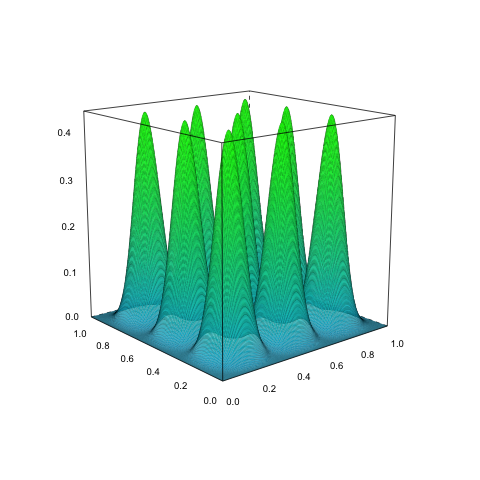
\includegraphics[width=4in,height=4in]{sparse_bicubic_basis.png}
  \caption{Landscape of cubic B-splines, a portion of a full bivariate basis}\label{fig:sparse_bicubic_basis}
\end{figure}

\subsubsection{{\outlineskeleton Computation}}

It is computationally efficient to express the surface in ``unfolded'' notation. Denote the support coordinate matrix  $C = \left(v \otimes \bfone_{\tilde{p}}, \bfone_p \otimes \tilde{v}\right)$ of dimension $p\tilde{p} \times 2$. Let $B_1$ and $B_2$ denote the matrices of dimensions $p\tilde{p} \times n$ and $p\tilde{p} \times \tilde{n}$ with entries corresponding to the univariate B-spline bases evaluated at each entry of the first and second column of $C$, respectively. {\needsparaphrased The unfolded expression at the support coordinates then has the standard multiple regression form}

\begin{equation} \label{eq:coef_surface_vec_notation}
\textup{vec}\left\{\alpha\left(t, \tilde{t}\right)\right\} = T^*\gamma
\end{equation}
\noindent
 where $\gamma = \textup{vec}\left(\Gamma\right)$. Define $T^*$ to be the matrix that is the result of taking the element-wise product of the matrices $\left(B_1 \otimes \bfone_n^\prime \right)$ and $\left(\bfone_{\tilde{n}}^\prime \otimes B_2 \right)$, written
\begin{equation}
T^*  = \left(B_1 \otimes \bfone_n^\prime \right) \odot \left(\bfone_{\tilde{n}}^\prime \otimes B_2 \right)
\end{equation} 
 \noindent 
where $\otimes$ denotes the Kronecker product operator. 

\subsection{{\outlineskeleton Penalized Two-Dimensional Coefficient Surfaces}}

Let $X_i = \left[x_{ijk}\right]$ denote the $i^{th}$ matrix of regression covariates, having dimension $p \times \tilde{p}$. Given $X_i$, the signal regressor support matrix $C$, and the corresponding coefficient surface $\alpha\left(t,\tilde{t}\right)$, we express the mean function 

\begin{equation} \label{eq:mean_regression_function}
\mu_i = \sum_{j=1}^p \sum_{k=1}^{\tilde{p}} x_{ijk} \alpha\left(t_j,\tilde{t}_k\right)
\end{equation} 
\noindent
where $i=1, \dots, m$, $j=1, \dots, p$, and $k=1,\dots,\tilde{p}$. Substituting \ref{eq:coefficient_surface_expansion} into \ref{eq:mean_regression_function}, we can expression the mean regression function in terms of the B-spline basis expansion:
\begin{equation} \label{eq:mean_regression_function_vec_notation}
\mu_i = \sum_{j=1}^p \sum_{k=1}^{\tilde{p}} x_{ijk}  \sum_{r=1}^n \sum_{s=1}^{\tilde{n}}  B_r\left(t_{j}\right) B_s\left(\tilde{t}_{k}\right) \gamma_{rs} = \bfx^\prime T^* \gamma
\end{equation} 
\noindent  
where $\bfx_i^\prime = \textup{vec}\left(X_i\right)$. A straightforward goodness of fit measure is the squared norm of the residual vector:

\begin{equation} 
\mathcal{Q}\left(\gamma\right) = \vert y - \bfX T^*\gamma \vert^2 = \vert y - M\gamma \vert^2  \label{eq:bivariate_resi_sum_of_squares}
\end{equation}
\noindent
where we define $M = \bfX T^*$, and $\bfX$ is the $m \times p\tilde{p}$ matrix of vectorized regressors, $\bfx_i$, $i=1,\dots,m$. While expressing the coefficient surface in terms of the tensor product B-splines reduces the model dimension, there are still $n\tilde{n}$ unknown parameters to be estimated from the data. Even moderately complex surfaces may require increasing the number of knots on the grid to allow enough flexibility for adequate estimation. There may also be regions without measurements, leading to a sparse $\bfX$, containing many zeros. Imposing structure through a regularization term will alleviate these potential issues.

{\needsparaphrased In the spirit of P-splines as discussed in section \ref{uni_pspline_penalties}, discrete roughness or difference penalties are imposed on $\Gamma$. Although we implement penalization on the vector form of coefficients ?, the motivation and mechanics of penalization is perhaps best seen through the matrix of coefficients ?. In fact a separate difference penalty is assigned to each of its rows and each of its columns. The penalties have structure to effectively break the linkage in the penalty from row to row or from column to column. The objective function is now modified, using penalties, to minimize }
\begin{equation} \label{eq:tensor_diff_penalty_obj_function_in_words}
\mathcal{Q}_\lambda\left(\gamma\right) = \textup{goodness of fit measure} + \textup{row penalty} + \textup{column penalty}
\end{equation}
\noindent
We choose to measure the fit of the coefficient surface using the residual sums of squares. This specification permits ease of computation, particularly when the penalty function can be expressed as a quadratic function of the unknown parameters. The objective function is indexed by $\lambda = \left(\lambda_1, \lambda_2\right)$, which are penalty parameters which control the complexity of the fitted surface. To facilitate smoothness across both dimensions of the coefficient surface, the penalty term is comprised of two parts: one which places a difference penalty on the rows of $\Gamma$, and the second imposes the difference penalty on the columns of $\Gamma$. Specifically, we define $\hat{\gamma}$ to be the minimizer of 

\begin{equation} \label{eq:bivariate_squared_diff_penalized_obj_function}
\begin{split}
\mathcal{Q}_\lambda\left(\gamma\right) &= \sum_{i=1}^m \left( y_i - \mu_i \right)^2 + \lambda_1 \sum_{r=1}^{n} \gamma_{r\bullet}^\prime D_k^\prime D_k \gamma_{r\bullet} 
+ \lambda_2 \sum_{s=1}^{\tilde{n}} \gamma_{\bullet s}^\prime D_{\tilde{k}}^\prime D_{\tilde{k}} \gamma_{\bullet s} \\
&= \sum_{i=1}^m \left( y_i - \sum_{j=1}^p \sum_{k=1}^{\tilde{p}} x_{ijk} \alpha\left(t_j,\tilde{t}_k\right) \right)^2 + \lambda_1 \sum_{r=1}^{n} \gamma_{r\bullet}^\prime D_k^\prime D_k \gamma_{r\bullet} + \lambda_2 \sum_{s=1}^{\tilde{n}} \gamma_{\bullet s}^\prime D_{\tilde{k}}^\prime D_{\tilde{k}} \gamma_{\bullet s} \\
 &=  \vert y - \bfX T^*\gamma \vert^2  + \lambda_1 \sum_{r=1}^{n} \gamma_{r\bullet}^\prime D_k^\prime D_k \gamma_{r\bullet} 
+ \lambda_2 \sum_{s=1}^{\tilde{n}} \gamma_{\bullet s}^\prime D_{\tilde{k}}^\prime D_{\tilde{k}} \gamma_{\bullet s}\\
 &=  \vert y - M\gamma \vert^2  + \lambda_1\vert P_1 \gamma \vert^2 + \lambda_2 \vert P_2 \gamma \vert^2 
\end{split}
\end{equation}
\noindent
where $\gamma_{r\bullet}$ and $\gamma_{\bullet s}$ denote the $r^{th}$ row and $s^{th}$ column of $\Gamma$, respectively. Kronecker products and matrix notation allow for compact representation of each of the components of the penalty:
\begin{equation} \label{eq:bivariate_squared_diff_penalty_projection_notation}
\begin{split}
P_1 &= \left( D_{k}^\prime D_k \right)\otimes I_{\tilde{n}}\\
P_2 &= I_{n}\otimes \left( D_{\tilde{k}}^\prime D_{\tilde{k}} \right)
\end{split}
\end{equation}
\noindent
where $I_{d}$ denotes the $d \times d$ identity matrix; $k$ and $\tilde{k}$ denote the orders of the difference penalties imposed on the column and row dimensions, respectively. $P_1$ and $P_2$ have corresponding fixed dimensions $\big[ \tilde{n} \left( n-k \right) \big] \times n\tilde{n}$ and $\big[ n \left(\tilde{n}-\tilde{k} \right) \big] \times n\tilde{n}$. In principle, the order of the differences in the penalty term can be considered as additional hyper-parameters, but in practice are typically fixed by the user, as one would typically fix the order of the differencing as one fixes the order of the squared derivative, as in the specification of the ridge regression penalty, for example. Further discussion of this topic will be presented in sections to follow.

\ref{eq:bivariate_squared_diff_penalized_obj_function} relies on two non-negative penalty parameters $\lambda_1$ and $\lambda_2$. These parameters allow for what can practically be viewed as continuous control of the smoothness of the surface in each dimension: the row dimension and the column dimension. This gives added flexibility, allowing for different degrees of smoothness across rows and columns. Figure 6 displays a possible scenario resulting from strong row (top panel) and strong column (bottom panel) penalization using a second order penalty on each row and column with large $\lambda_1$ and $\lambda_2$. Notice that the limiting behavior for each row and column is linear, but reversals of slopes are possible from one row (or column) to the next.

An example of a first and second order penalty matrix $D$ for small $n = \tilde{n} = 3$ (for one row or column of $\Gamma$) looks like

\[
D_1 = \begin{bmatrix} 
-1 & 1 & 0 \\
0 & -1 & 1 
\end{bmatrix}
\quad
D_2 = \begin{bmatrix} 
1 & -2 & 1 
\end{bmatrix}
\]
Each row and column of $\Gamma$ has its own banded differencing matrix, $D$, so that the projection onto the penalized column space has structure
\[
P_1 = \begin{bmatrix} 
1 & 0 & 0 \\
0 & 1 & 0\\ 
0 & 0 & 1\\ 
\end{bmatrix} \otimes D_1 = \left[ \begin{array}{ccccccccccc}  -1 & 1 & 0  & &  0 & 0 & 0 &  &  0 & 0 & 0  \\
						0 & -1 & 1 & & 0 & 0 & 0 &  &  0 & 0 & 0  \\ 
						&&&&&&&&&&\\
						0 & 0 & 0  & & -1 & 1 & 0  & & 0 & 0 & 0  \\ 
						0 & 0 & 0  & & 0 & -1 & 1 & & 0 & 0 & 0  \\ 
						&&&&&&&&&&\\
						0 & 0 & 0  & & 0 & 0 & 0 &  & -1 & 1 & 0  \\
						0 & 0 & 0  & & 0 & 0 & 0 &  &  0 & -1 & 1  
						\end{array} \right] 
\]
\noindent 
and the projection operator corresponding to the row penalty is of the form
\[
P_2 = D_1 \otimes \begin{bmatrix} 
					1 & 0 & 0 \\
					0 & 1 & 0\\ 
					0 & 0 & 1\\ 
					\end{bmatrix} = \left[ \begin{array}{ccccccccccc}  -1 & 0 & 0  & &  1 & 0 & 0 &  &  0 & 0 & 0  \\
														   0 & -1 & 0 & & 0 & 1 & 0 &  &  0 & 0 & 0  \\ 
														   0 & 0 & -1  & & 0 & 0 & 1  & & 0 & 0 & 0  \\ 
														   &&&&&&&&&&\\					
														   0 & 0 & 0  & & -1 & 0 & 0 &   & 1 & 0 & 0  \\ 
														   0 & 0 & 0  & & 0 & -1 & 0 &  & 0 & 1 & 0  \\
														   0 & 0 & 0  & & 0 & 0 & -1 &  &  0 & 0 & 1  
														  \end{array} \right] 
\]

One should also note that this formulation allows for seamless accommodation of different orders of differencing for rows and columns. 

Taking derivatives of \ref{eq:bivariate_squared_diff_penalized_obj_function} with respect to $\gamma$, we have
\begin{eqnarray*}
\frac{\partial}{\partial \gamma}\mathcal{Q}_{\lambda}\left(\gamma\right)&=& \bigg[M^\prime M + \lambda_1P_1^\prime P_1 + \lambda_2P_2^\prime P_2 \bigg]\gamma - M^\prime y
\end{eqnarray*}
\noindent
and setting equal to zero, yields the explicit $P$-spline estimator

\begin{equation} \label{eq:pspline_estimator}
\hat{gamma} = \left( M^\prime M + \lambda_1 P_1^\prime P_1 + \lambda_2 P_2^\prime P_2\right)^{-1}M^\prime y
\end{equation}

{\needsparaphrased The predicted response values are then given by $\hat{y} = M\hat{\gamma}$, and the effective hat matrix is}

\begin{equation} \label{eq:bivariate_pspline_hat_matrix}
H = M\left( M^\prime M + \lambda_1 P_1^\prime P_1 + \lambda_2 P_2^\prime P_2\right)^{-1} M^\prime
\end{equation}

An attractive feature of this estimator is that the dimension of the system of normal equations remains fixed at $n\tilde{n}$ even while the resolution of the observation grid, $p\tilde{p}$, increases. The solution can be easily modified to include an intercept term, $\alpha_0$ and its corresponding penalty. Additionally, one may include an overall ridge penalty:

\[
\lambda_0 \vert \gamma \vert^2, \quad \lambda_0 > 0
\] 

To accommodate an intercept term, one simply augments the modified design matrix with a vector of ones, letting $\breve{M} = \left[ \bfone \vert M \right]$. Letting $\breve{P}_i = \left[ \bfo \vert\right]$ for $i=1,2$, and $\breve{I} = \textup{diag}\left(\bfo, I_{n\tilde{n}}\right)$, the modified estimator is given by 

\begin{equation*}
\left( \hat{\alpha}_0, \hat{\gamma}^\prime \right)^\prime = \left( \breve{M}^\prime \breve{M} + \lambda_1 \breve{P}_1^\prime \breve{P}_1 + \lambda_2 \breve{P}_2^\prime \breve{P}_2 + \lambda_0\breve{I}\right)^{-1}\breve{M}^\prime y
\end{equation*} 
\noindent
where the addition of the zero vectors to the penalty projection matrices and the identity matrix ensure that the intercept term is not penalized. Advantages of this approach is that we sidestep the choice of the number and placement of the spline knots, which is a difficult optimization problem in itself. The penalty terms introduce little additional computational complexity, since the smoothing parameters have no impact on $\tilde{M}^\prime M$ and $\tilde{M}^\prime y$ and thus do not need to be recomputed when these parameters are varied. For fixed $k$, as $\lambda_i$, $i=1,2$ increases $\gamma$ becomes smoother in its corresponding dimension, approaching a polynomial of degree $k-1$. As the hat matrix is easily obtained, leave-one-out cross validation   error estimates are also easy to obtain.  



















\subsection{Nonparametric approaches to modeling nonlinear time series data}

Zeger and Diggle (1994) present a partially linear model motivated by the longitudinal data produced by the Multicenter AIDS Cohort Study. The data are of the form $\left\{ \left(x_{ij},y_{ij}\left(t_{ij}\right)\right): \;\; j=1,\dots,m_i;\;\;i=1,\dots,n \right\}$, where $x_{ij}$ denotes a $p \times 1$ vector of covariates corresponding to $y_{ij}\left(t_{ij}\right)$, the $j$th measurement on the $i^{th}$ subject at time $t_{ij}$. They let 

\begin{equation} \label{eq:zeger_diggle_VC_model}
Y_{ij}\left(t\right) =  x_{ij}^T\beta + \mu\left(t\right) + W_i\left(t\right) + \epsilon_{ij}
\end{equation}
\noindent
where $\mu\left(t\right)$ is a smooth function of time, and $\beta$ is a $p \times 1$ vector of regression coefficients. The $\left\{ W_i\left(t\right):\;i=1,\dots,n \right\}$ capture the within-subject dependency structure, defined to be independent replicates of a stationary Gaussian process with mean zero and covariance function $\gamma\left(v\right) = \sigma_w^2\rho\left(v, \theta \right)$. The $\left\{ Z_{ij}:\;j=1,\dots,m_i\;i=1,\dots,n \right\}$ are mutually independent Normally distributed error terms with mean zero and variance $\sigma_z^2$.

Hoover, Rice, Wu and Yang (1998) considered the following model:

\begin{equation} \label{eq:hoover_rice_wu_VC_model}
Y\left(t\right) =  \bfX^T\left(t\right)\bfbeta \left(t\right) + \epsilon\left(t\right) 
\end{equation}
\noindent
proposing estimation of the coefficient functions via smoothing splines and local polynomials. $\epsilon\left(t\right)$ is defined as in \ref{eq:zeger_diggle_VC_model} and is assumed to be independent of $\bfX\left(t\right)$. Hoover et al (1998) propose the same model, using smoothing splines and kernel smoothing to estimate  the components of $\bfbeta\left(t\right)$ and develop asymptotic properties of kernel estimators. 



For nonlinear time series applications, Chen \& Tsay \cite{chen1993functional} and Xia \& Li (1999) develop functional-coefficient autoregressive models. The common research in nonlinear time series analysis has focused on several classes of models, such as the threshold autoregressive (TAR) model of Tong (1983, 1990) and the exponential autoregressive (EXPAR) model of Haggan and Ozaki (1981). {\needsparaphrased In this article we are concerned with empirical modeling of nonlinear time series. In particular we focus on exploring the nonlinear feature of a time series in the process of model building. This is achieved by generalizing directly the linear autoregressive (AR) models and exploiting local characteristics of a given time series. The generalized model is referred to as the functional coefficient autoregressive (FAR) models. Most nonlinear AR models considered in the literature are special cases of the FAR model. It turns out that the FAR models are flexible enough to accommodate most nonlinear features considered in the literature while being simple enough to be treated with relative ease. }


\section{Model estimation}

Zeger and Diggle (1994) carry out estimation of $\mu\left(t\right)$ and $\beta$ as defined in model \ref{eq:zeger_diggle_VC_model} iteratively via kernel smoothing and generalized least squares. While more flexible than the classical linear model, this still limiting as it does not allow us to explain any dynamic effect of the covariates over time.  


In the case of a single common smoothing variable, estimation of \ref{eq:VC_mean_function_single_smoothing_covariate} via kernel smoothing is quite straightforward. Since the space of the smoothing variable is of only one dimension, smoothing of the $p$ coefficient functions reduces to finding the local least squares fit using a single smoothing bandwidth. This approach, however, may lead to inadequate estimators since the functions $\beta_0\left(z\right), \beta_1\left(z\right), \dots, \beta_p\left(z\right)$ may need varying degrees of smoothing in the $z$ dimension. To address this, 

\subsection{Kernel estimation with a single smoothing variable}

Suppose we have a random sample of data, consisting of $\left\{ \left(x_1, y_1\right),\dots, \left(x_n, y_n\right)\right\}$, for $i=1,\dots,n$. In classical univariate nonparametric regression, we model 

\begin{equation}
Y_i = f\left(x_i\right) + \epsilon_i,\;\;\;i=1,\dots, n \label{eq:classical_NP_regression_model}
\end{equation} 
\noindent
where $f$ is the unknown smooth regression function of interest, and the $\left\{ \epsilon_i \right\}$ are mutually independent mean-zero errors, with $Var\left(\epsilon_i\right)=\sigma_\epsilon^2$. To derive the form of the estimator of the mean function, we consider expressing $f$ in terms of the joint probability distribution of $X$ and $Y$:

\begin{eqnarray} 
f\left(x\right) = E\left(Y \vert X=x\right) &=& \int yp(y \vert x)\;dy \nonumber \\
&=& \frac{ \int yp(y \vert x)\;dy }{ \int p(y \vert x)\;dy } \label{eq:conditional_mean_y_given_x}
\end{eqnarray}
 
Let $K$ denote a kernel function corresponding to a probability density, $h$ denote the smoothing bandwidth, and let 

\[
K_h\left(t\right) = h^{-1} K\left(h^{-1} t \right)
\] 

The Nadaraya-Watson estimator of the joint density of $x$ and $y$ has form

\begin{eqnarray} 
\hat{p}\left(x,y\right) &=& \frac{1}{nh_x h_y}\sum_{i=1}^{n} K_{h_x}\left(\frac{x-x_i}{h_x}\right) K_{h_y}\left(\frac{y-y_i}{h_y}\right)  \nonumber \\ 
&=& \frac{1}{n}\sum_{i=1}^{n} K_{h_x}\left(x-x_i\right) K_{h_y}\left(y-y_i\right) \label{eq:NW_joint_pdf_estimator} 
\end{eqnarray}
\noindent
Then, substituting \ref{eq:NW_joint_pdf_estimator} for $p\left(x,y\right)$ in the numerator of \ref{eq:conditional_mean_y_given_x}, we can write 

\begin{equation} \nonumber 
\int y \hat{p}\left(x,y\right)\;dy = \frac{1}{n} \int y K_{h_x}\left(x-x_i\right) K_{h_y}\left(y-y_i\right)
\end{equation} 
\noindent
Since $\int yK_{h_y}\left(y-y_i\right)dy = y_i$, we have that 
\begin{equation} \label{eq:num_est}
\int y \hat{p}\left(x,y\right)\;dy = \frac{1}{n}\sum_{i=1}^n K_{h_x}\left(x-x_i\right) y_i 
\end{equation} 
\noindent
Estimating the denominator of \ref{eq:conditional_mean_y_given_x} in similar fashion, we have 

\begin{eqnarray}
\int \hat{p}\left(x,y\right)\;dy &=& \frac{1}{n}\sum_{i=1}^{n} K_{h_x}\left(x-x_i\right) \int K_{h_y}\left(y-y_i\right)\;dy \nonumber \\
&=& \frac{1}{n}\sum_{i=1}^{n} K_{h_x}\left(x-x_i\right) \nonumber \\
&=& \hat{f}_x\left(x\right) \label{eq:den_est} 
\end{eqnarray}

Using \ref{eq:num_est} and \ref{eq:den_est} as plug-in estimators in \ref{eq:conditional_mean_y_given_x}, then 

\begin{equation} 
\hat{f}\left(x\right) = \sum_{i=1}^n W_{h_x}\left(x,x_i\right)y_i
\end{equation}
\noindent
where 
\begin{equation} \nonumber
W_{h_x}\left(x,x_i\right) = \frac{K_{h_x}\left(x-x_i\right) }{\sum_{i=1}^{n} K_{h_x}\left(x-x_i\right)}
\end{equation}
\noindent
and $\sum_{i=1}^n W_{h_x}\left(x,x_i\right) = 1$. One can extend this to the case where the regression function is defined as in \ref{eq:VC_mean_function_single_smoothing_covariate}; the Nadaraya-Watson (NW) estimator of $\bfbeta\left(z_0\right) = \left(\beta_0\left(z_0,\right), \beta_1\left(z_0,\right),\dots,\beta_p\left(z_0,\right)\right)^T$ minimizes

\begin{equation} \nonumber 
\sum_{i=1}^n \left(Y_i - \left(\sum_{j=1}^p \alpha_j X_{ij}\right)\right)^2 K_{h_z}\left(z_0,Z_i\right)
\end{equation} 
\noindent
with respect to $\bfalpha = \left( \alpha_1, \dots, \alpha_p\right)^T$ for each target point $z_0$. Let $\mathcal{X}$ denote the $n \times p$ matrix having $i-j^{th}$ element $X_{ij}$, $\mathcal{W}$ denote the $n \times n$ diagonal matrix with $i^{th}$ diagonal entry $K_{h_z}\left(z_0, Z_i\right)$, and let $\bfZ = \left(Z_1, \dots, Z_n\right)^T$. Further, let $\bfY = \left(Y_1, \dots, Y_n\right)^T$, then the NW estimator has form

\begin{equation} \nonumber
\hat{\bfbeta}\left(z_0\right) = \big[\mathcal{X}^T\mathcal{W}\mathcal{X}\big]^{-1} \mathcal{X}^T\mathcal{W} \bfY
\end{equation} 


It is well known that locally weighted averages can exhibit high bias near the boundaries of the smoothing variable domain, due to the asymmetry of the kernel in that region. This bias can also be present on the interior of the domain when the observed values of $Z$ are irregularly sampled, though it is typically less severe in the interior than near the boundaries. To remedy this, one may consider fitting local linear smoothers, which will correct this bias to first order. The local linear smoother minimizes 

\begin{equation} \label{local_linear_smoother_obj_fun} 
\sum_{i=1}^n \Big[Y_i - \sum_{j=1}^p \left(\alpha_{0j}+\alpha_{1j}\left(Z_i - z_0 \right)\right)X_{ij}\Big]^2 K_{h_z}\left(z_0,Z_i\right)
\end{equation} 
 
 \noindent
 with respect to $\bfalpha_0 = \left( \alpha_{01}, \dots, \alpha_{0p}\right)^T$, and $\bfalpha_1 = \left( \alpha_{11}, \dots, \alpha_{1p}\right)^T$. Let $\mathcal{X}$ denote the $n \times 2p$ matrix having $i-j^{th}$ element $X_{ij}$ and $i-\left(j+p\right)^{th}$ element $\left(Z_i - z_0\right)X_{ij}$ for $1 \le  j \le p$, then the minimizer of \ref{eq:local_linear_smoother_obj_fun} is given by 
 
\begin{equation} \nonumber
\hat{\bfbeta}\left(z_0\right) = \big[ \mathcal{I}_p, \bfO_p \big]\big[\mathcal{X}^T\mathcal{W}\mathcal{X}\big]^{-1} \mathcal{X}^T\mathcal{W} \bfY
\end{equation}   

\noindent
where $\mathcal{I}_p$ is the $p \times p$ identity matrix, and $\bfO_p$ is the $p \times p$ zero matrix. Extensions to the case of a single multivariate smoothing variable $\bfZ$, where the mean function is given by 

\[
E\left(Y \vert \bfX=\bfx, \bfZ=\bfz \right) = x_1\beta_1\left(\bfz\right) + \dots  + x_p\beta_p\left(\bfz\right)
\]
\noindent
However, while boundary effects associated with the NW estimator are a concern in one dimension, the curse of dimensionality makes these effects much more problematic in two or more dimensions. The fraction of points close to the boundary of the domain approaches one as the dimensionality of the input space grows, and simultaneously maintaining locality (and low bias) as well as sizable number of observations in the neighborhood of the target point, $z_0$ (low variance) becomes an increasingly tall order. 

\subsubsection{Kernel bandwidth selection with a single smoothing variable} \label{single_smoothing_var_bandwidth_selection}
\subsubsection{Asymptotic properties of kernel estimators with a single smoothing variable}

\subsubsection{Two-step estimation for multiple bandwidths} \label{two_step_kernel_smoothing}

Model selection as described in \ref{single_smoothing_var_bandwidth_selection} assumes a single smoothing bandwidth $h_z$ as well as a single common kernel function $K$ for every coefficient function $\beta_j$. While convenient and straightforward, in practice, the assumption that each coefficient function should receive the same degree of smoothing is likely to be an erroneous one. Fan and Zhang (1999) present an intuitive formulation of their proposed two-stage estimation procedure that allows for each coefficient function to have its own smoothing bandwidth. Assume that $\beta_p\left(z\right)$ is smoother than the other $p-1$ coefficient functions, and can be locally approximated by a cubic polynomial:

\[
\beta_p\left(z\right) \approx b_{0p} + b_{1p} \left(z-z_0\right) + b_{2p} \left(z-z_0\right)^2 + b_{3p} \left(z-z_0\right)^3
\] 
\noindent 
for any $z_0$ close to $z$. Let $\left\{ \tilde{b}_{0j}, \tilde{b}_{1j} \right\}$, $j=1,\dots, p-1$ and $\tilde{b}_{0p}, \tilde{b}_{1p}, \tilde{b}_{2p}, \tilde{b}_{3p}$ be the minimizers of the weighted sums of squares:

\begin{IEEEeqnarray*}{lll}
\sum_{i=1}^n \Big[ Y_i &-& \sum_{j=1}^{p-1}\left\{ b_{0j} + b_{1j}\left(Z_i-z_0\right) \right\} X_{ij} \\ 
&-& \left\{ b_{0p} + b_{1p} \left(z-z_0\right) + b_{2p} \left(z-z_0\right)^2 + b_{3p} \left(z-z_0\right)^3 \right\} X_{ip} \Big]^2 \times\> K_{h_1}\left(Z_i-z_0\right)
\end{IEEEeqnarray*}

If we take $\tilde{\beta}^{os}_p\left(z_0\right) = \tilde{b}_{0p}$, then they show that the bias of the the \textit{one-step estimator} is $O\left(h_0^2\right)$ and the variance is $O\left( \left(nh_0 \right)^{-1} \right)$. Fan and Zhang (1999) propose a two-step estimation procedure that allows for individual degrees of smoothing of each of the coefficient functions; Cai (2000) further investigated this two-step approach. In the first step, to estimate $\beta_j\left(z_0\right)$, a preliminary estimate, $\tilde{\beta}_j$, is obtained by applying a local cubic smoother to $\beta_j$ and local linear smoothing to the remaining $p-1$ functions with a single common bandwidth, $h_0$, for every $j$. In the second step, a local cubic smoother is again applied to the residuals $Y_i-\sum_{j\ne k} X_{ik} \tilde{\beta}\left( z_0 \right)$ using function-specific bandwidth to obtain the final estimate of $\beta_j\left(z_0\right)$. They present the asymptotic mean-squared error of the estimates obtained by this procedure, and further show  that the estimates achieve optimal convergence rates. Cai (2000) demonstrated that even when every coefficient function exhibits the same degree of smoothness, the two-step estimates exhibit the same asymptotic properties as the usual one-step local smoother.  

\subsection{Kernel estimation with multiple smoothing variables}

A proposed extension of model \ref{eq:VC_mean_function_single_smoothing_covariate} permits each coefficient function to depend on its own smoothing variable: 

\begin{equation} \nonumber
E\left(Y \vert \bfX=\bfx,\;Z = z \right) = x_1\beta_1\left(z_1\right) + \dots  + x_p\beta_p\left(z_p\right)
\end{equation}

While the expression of the model itself does not make this obvious, estimation of this model is significantly different than the estimation of the model assuming a single common smoothing parameter for every coefficient function. Xue \& Yang (2006a) further generalized this model where each coefficient function is replaced by a multivariate function with additive structure:

\begin{equation} \label{eq:VC_mean_MV_function_multiple_smoothing_covariates}
E\left(Y \vert \bfX=\bfx,\;\bfZ = \bfz \right) = x_1\sum_{j=1}^q \beta_{1j}\left(z_1\right) + \dots  + x_p\sum_{j=1}^q \beta_{pj}\left(z_p\right)
\end{equation}
\noindent
which allows for inclusion of all interaction terms $X_j \beta_{jk}\left(Z_k\right)$, $j=1,\dots,p$, $k=1,\dots, q$. Applying multivariate kernel smoothing locally to each point $\bfz = \left(z_1,\dots,z_p \right)^T$ results in multivariate functions of the entire covariate vector, losing the structure of model \ref{eq:VC_mean_function_multiple_smoothing_covariates}. To extract proper estimates of the $\left\{  \beta_j \right\}$, two primary methodologies have been proposed: marginal integration and smooth backfitting. Linton and Nielsen (1995) employ local kernel smoothing to estimate the multivariate coefficient functions $\left\{ \beta_j\left( \bfz\right) \right\}$, minimizing

\[
n^{-1} \sum_{i=1}^n \left( Y_i  - \sum_{j=1}^q \alpha_j X_{ij} \right)^2 K_{h_1}\left(z_1,Z_{i1}\right) \times \dots \times K_{h_p}\left(z_p,Z_{ip}\right)
\]
\noindent
for each value of $\bf$. Integrating the multivariate coefficient functions over the support of the smoothing variables gives marginal estimates of $\beta_j$. This approach, however, suffers from the curse of dimensionality, as the attractive statistical properties of the estimators $\hat{\beta}_j$ depend heavily on the consistency of the $\left\{ \alpha_j \right\}$, which requires $n\times h_1\times \dots \times h_p \rightarrow \infty$, thus losing the attractive qualities of local methods. The smooth backfitting method initially introduced by Mammen et al. (1999) for additive regression models enjoys both theoretical and numerical advantages over the integration method, and is free of the curse of dimensionality. To estimate $\left\{ \alpha_j \right\}$, one minimizes the integrated weighted sum of squares

\[
\int n^{-1} \sum_{i=1}^n \left( Y_i - \sum_{j=1}^p \alpha_j\left(z_j\right) \right)^2 K_{h_1}\left(z_1,Z_{i1}\right) \times \dots \times K_{h_p}\left(z_p,Z_{ip}\right) \;d\bfz
\]
\noindent
over the space of function tuples $\mathcal{H} = \left\{ \bfalpha = \left(\alpha_1,\dots, \alpha_p\right):\alpha_j\left(\bfz\right) = \alpha_j\left(z_j\right) \right\}$, so that the optimization must not be performed for every $\bfz$. For a detailed discussion of these methods, we refer the reader to Linton and Nielsen (1995) and Mammen \& Park (2005). 





\subsection{Basis expansions and penalized likelihood techniques} \label{VC_spline_models}

In classical nonparametric regression problems, $m\left(x\right) = E\left(Y\vert X\right)$ is represented by a linear basis expansion in $X$, so that

\[
E\left(Y \vert X\right) = \sum_{j=1}^M \beta_m b_m\left(X\right)
\]
\noindent
with $M \rightarrow \infty$. The general estimation framework may be described as follows: The estimation space, $G = G_n$, is the linear space of bounded functions having finite dimension $M_n$. For a given loss function $\mathcal{L}$, the estimate of $m$, $\hat{m}$, is defined to be the element of $G_n$ which minimizes $\mathcal{L}$ and maybe be characterized by the estimates of the basis function coefficients $\beta_1,\dots, \beta_m$. It is typical that the true mean function does not belong to $G_n$, and members of $G_n$ are taken to be an approximation to the truth. Typical choices for loss functions include sums of squared errors or negative log likelihood functions. To this end, it is natural to allow the dimension of the estimation space to grow with the sample size. The choice of basis is not a trivial one, and some choices include logarithms, power functions, or wavelets; there is, however, disadvantages to using basis functions with unrestricted support. Piecewise polynomials and splines are families of functions with each member of which having bounded support. This allows for local representations of $m\left(x\right)$, while still permitting ease of implementation, as their estimation is carried out through the global optimization of $\mathcal{L}$. 

These methods in the classical setting have been explored extensively; Chen (2007) provides an extensive review of the asymptotic behaviour of these estimators. Zhou, Shen, and Wolfe (1998) establish asymptotic normality of univariate regression splines; they present explicit expressions for the asymptotic pointwise bias and variance of the estimator, providing a method of constructing confidence intervals and confidence regions when the knots are asymptotically equally spaced and are distributed according to a continuous density. Their results additionally require that the order of the spline is equal to the order of the derivative of the unknown function to be estimated. Huang et al. (2003) establish asymptotic results for not only the univariate case, but also for tensor product splines and multivariate splines on triangulations.  

A general representation of models \ref{eq:VC_mean_function_single_smoothing_covariate}, \ref{eq:VC_mean_function_multiple_smoothing_covariates}, and \ref{eq:VC_mean_MV_function_multiple_smoothing_covariates} may be represented as follows:

\begin{equation} \label{eq:general_VC_model}
E\left(Y \vert \bfX, \bfZ\right) = \sum_{i=1}^q \bfX_i^T \bfbeta_i\left(\bfZ_i\right)
\end{equation}
\noindent
where $\bfX_i$ is a $d_i \times 1$ vector, $d_i \ge 1$; $\bfX$ is the collection of all covariates contained in $\left\{ \bfX_i \right\}$, $i=1,\dots,q$. For example, model \ref{eq:VC_mean_MV_function_multiple_smoothing_covariates} may be written as above by letting $\bfX_i \equiv \bfX = \left(X_1,\dots, X_p\right)^T$ for every $j$. The majority of the work in this area has been for the case where $q=1$.  Xue and Yang (2005a) allowed for multivariate coefficient functions, assuming an additive structure by letting

\begin{eqnarray} 
E\left(Y \vert \bfX, \bfZ\right) &=& \sum_{i=1}^{d_1} X_i \beta_i\left(\bfZ\right) \label{eq:xue_VC_model}\\
\beta_i\left(\bfZ\right) &=& \sum_{j=1}^{d_2} \beta_{ij}\left(Z_j\right) \nonumber
\end{eqnarray}
\noindent
for $i=1,\dots, d_1$.

 

















\subsection{Smoothing methods with longitudinal data}

Models \ref{eq:VC_mean_function_single_smoothing_covariate}, \ref{eq:VC_mean_function_multiple_smoothing_covariates}, and \ref{eq:VC_mean_MV_function_multiple_smoothing_covariates} can be written as follows:

\begin{equation} \label{eq:functional_VC_model}
Y\left(t\right) = \sum_{j=1}^q \bfX_j^T \bff \left(T\right) + \epsilon\left(T\right)
\end{equation}

where $\bff = \left(f_1,\dots, f_q \right)^T$ is the vector of coefficient functions of interest and $\epsilon\left(t\right)$ is a mean zero stochastic process. Both the response and covariates are assumed to be observed at subject-specific times, which may be irregularly spaced. Let $\bfX_{ij} = \bfX_i\left(T_{ij}\right)$ and $Y_{ij} = Y_i\left(T_{ij}\right)$ denote the observed covariates and responses on subject $i$ at random time points $\left\{ T_{ij} \right\}$, $j=1,\dots,n_i$. Given this structure, model  \ref{eq:functional_VC_model} can be written 
   
\begin{equation} \label{longitudinal_VC_model}
Y_{ij} = \bff\left(T_{ij}\right)^T\bfX_{ij} + \epsilon_{ij}
\end{equation}
\noindent
where $\epsilon_{ij} = \epsilon\left(T_{ij}\right)$. The $\left\{ T_{ij} \right\}$ are assumed to be independent for all $i,j$; $\bfX_{ij}$ and $\epsilon_{ij}$ are assumed to be independent across values of $i$, but may exhibit within-subject dependency structure.  A simple avenue of model estimation for model \ref{eq:longitudinal_VC_model} is to apply local smoothing, where the Nadaraya-Watson estimator minimizes 

\begin{equation} \label{eq:longitudinal_NW_objective_function}
N^{-1} \sum_{i=1}^{n} \sum_{j=1}^{n_i} \left(Y_{ij} - \sum_{k=1}^q \alpha_k X_{ijk} \right)^2 K_h\left(t,T_{ij}\right)
\end{equation}
\noindent

with respect to $\alpha = \left(\alpha_1,\dots, \alpha_q \right)^T$, where $N = \sum_{i=1}^n n_i$. The specification in \ref{eq:longitudinal_NW_objective_function} places equal weights on all subjects; to assign individual weights to each subject's contribution to the loss function, one may instead minimize

\begin{equation} \label{eq:longitudinal_NW_objective_function}
n^{-1} \sum_{i=1}^{n} w_i \sum_{j=1}^{n_i} \left(Y_{ij} - \sum_{k=1}^q \alpha_k X_{ijk} \right)^2 K_h\left(t,T_{ij}\right)
\end{equation}
\noindent 
where one may specify, for example, $w_i = n_i^{-1}$. Hoover et al. (1998) proposed kernel estimation using local polynomial smoothing, of which the minimization of \ref{eq:longitudinal_NW_objective_function} is a special case. Wu et al present the construction of both point-wise confidence intervals as well as simultaneous confidence regions based on the asymptotic normality of the local kernel smoother.

\bibliography{Master} 
%\bibliographystyle{amsplain}
\bibliographystyle{apalike}


\end{document}

